\documentclass[11pt,a4paper]{article}

% --- PACOTES ESSENCIAIS ---
\usepackage[utf8]{inputenc}
\usepackage[T1]{fontenc}
\usepackage[portuguese]{babel}
\usepackage{geometry}
\geometry{a4paper, top=2.5cm, bottom=2.5cm, left=2.5cm, right=2.5cm}

% --- PACOTES PARA GRÁFICOS E TABELAS (kableExtra e imagens) ---
\usepackage{graphicx}
\usepackage{booktabs}
\usepackage{longtable}
\usepackage{array}
\usepackage{multirow}
\usepackage{float}
\usepackage{colortbl}
\usepackage{xcolor}
\usepackage{textcomp}
\usepackage{threeparttable}
\usepackage[normalem]{ulem}
\usepackage{makecell}

% --- TIPOGRAFIA E FORMATAÇÃO ---
\usepackage{mathpazo}
\usepackage{setspace}
\usepackage{indentfirst}
\usepackage{etoolbox}
\usepackage[hidelinks]{hyperref}
\hypersetup{
  pdftitle = {Relatório Final (DHEM e Sarcopenia)},
  pdfauthor = {Lucas Batista de Oliveira}
}
\emergencystretch=3em

% Compatibilidade com longtable v4.24 (evita cola com retração infinita
% durante a divisão de tabelas entre páginas). Falhas não interrompem a compilação.
\makeatletter
\patchcmd{\LT@output}
{\copy\LT@foot\vss}
{\copy\LT@foot\vskip 0pt plus 1fil minus \maxdimen}
{\typeout{Longtable patch 1 ok}}{\typeout{Longtable patch 1 falhou}}
\patchcmd{\LT@output}
{\copy\LT@foot\vss}
{\copy\LT@foot\vskip 0pt plus 1fil minus \maxdimen}
{\typeout{Longtable patch 2 ok}}{\typeout{Longtable patch 2 falhou}}
\makeatother

% --- MACROS DINÂMICAS GERADAS PELO R (outputs/macros.tex) ---
\newcommand{\NTotal}{165}
\newcommand{\NSemDHEM}{22}
\newcommand{\NDHEMSemFibrose}{101}
\newcommand{\NDHEMComFibrose}{42}
\newcommand{\MediaIdade}{59,2}
\newcommand{\MedianaIdade}{61}
\newcommand{\MediaIMC}{32,2}
\newcommand{\DPIMC}{6,3}
\newcommand{\PercMulheres}{80,0\%}
\newcommand{\PercDHEM}{83,6\%}
\newcommand{\PercFibrose}{25,5\%}
\newcommand{\PercObesidade}{62,4\%}
\newcommand{\PercDiabetes}{73,3\%}
\newcommand{\PercHipertensao}{83,0\%}
\newcommand{\PercSarcSARCF}{27,3\%}
\newcommand{\PercSarcSARCFCC}{19,6\%}
\newcommand{\PercSarcHandgrip}{29,9\%}
\newcommand{\PercSarcElev}{47,8\%}
\newcommand{\PercSarcVel}{77,8\%}
\newcommand{\PercIMMABaixo}{15,2\%}
\newcommand{\PercIMMANewman}{44,8\%}
\newcommand{\PercIMMABaumgartner}{7,3\%}
\newcommand{\PercIMMAFNIH}{21,2\%}
\newcommand{\PercIMMAPeso}{7,9\%}
\newcommand{\PercSarcNewman}{13,3\%}
\newcommand{\PercSarcBaumgartner}{2,4\%}
\newcommand{\PercSarcFNIH}{7,9\%}

\newcommand{\ICIMMABaixoInf}{10,2}
\newcommand{\ICIMMABaixoSup}{21,7}
\newcommand{\ICIMMANewmanInf}{37,2}
\newcommand{\ICIMMANewmanSup}{52,8}
\newcommand{\ICIMMABaumgartnerInf}{4,0}
\newcommand{\ICIMMABaumgartnerSup}{12,6}
\newcommand{\ICIMMAFNIHInf}{15,4}
\newcommand{\ICIMMAFNIHSup}{28,4}
\newcommand{\ICIMMAPesoInf}{4,4}
\newcommand{\ICIMMAPesoSup}{13,4}
\newcommand{\KappaFleiss}{0,19}
\newcommand{\KappaFleissDHEM}{0,20}
\newcommand{\NDHEMConcord}{138}
\newcommand{\BetaFibroseMMT}{0,70}
\newcommand{\PBetaFibroseMMT}{0,452}


\begin{document}
\setstretch{1.15}

% ==============================================================================
% CABEÇALHO
% ==============================================================================
\begin{flushright}
  {\LARGE\bfseries Relatório Final}\\[0.4em]
  {\large Associação entre DHEM e Sarcopenia}\\[0.8em]
  {\normalsize Consultor: Lucas Batista de Oliveira}\\
  {\normalsize Requisitante: Jordanna de Paula Mendes Torres}\\
  {\normalsize Data de atualização: \today}
\end{flushright}

\vspace{0.6cm}
\begin{center}
  \textbf{Material desenvolvido para fins avaliativos na disciplina Prática
  Estatística III (GET00109).}
\end{center}

\vspace{0.6cm}
\tableofcontents
\vspace{0.6cm}
\hrule
\vspace{0.8cm}

% ==============================================================================
\section{Resumo do Projeto}
% ==============================================================================

Este relatório apresenta os resultados da consultoria estatística para o
projeto \textit{Disfunções Endócrinas em Pacientes com DHEM (Sub-projeto:
Sarcopenia)}, conduzido com dados reais do Ambulatório de Endocrinologia do
HUAP/UFF. O objetivo central é investigar a associação entre a doença hepática
esteatótica associada à disfunção metabólica (DHEM) e à sarcopenia, com ênfase
na ocorrência de degeneração muscular em pacientes com fibrose hepática.

A amostra analisada contou com \NTotal{} pacientes, com idade média de
\MediaIdade{} anos (mediana de \MedianaIdade{} anos) e IMC médio de \MediaIMC{}
kg/m$^2$ (DP = \DPIMC{}). Do total, \PercMulheres{} são do sexo feminino,
\PercDHEM{} apresentaram diagnóstico de DHEM e \PercFibrose{} apresentaram
fibrose hepática significativa. As prevalências de sarcopenia variaram conforme
o critério adotado, entre \PercSarcBaumgartner{} (critério de Baumgartner
combinado ao handgrip) e \PercSarcVel{} (velocidade de marcha $< 0{,}8$ m/s).

% ==============================================================================
\section{Contexto e Objetivos}
% ==============================================================================

\subsection{Contexto clínico}

A DHEM é uma das causas mais frequentes de doença hepática crônica e está
associada à obesidade, diabetes mellitus tipo 2 e síndrome metabólica. Estudos
recentes apontam uma relação bidirecional entre a DHEM e a sarcopenia: a perda
progressiva e generalizada de massa e força muscular esquelética pode agravar o
acúmulo de gordura hepática, enquanto a doença hepática avançada contribui para
a degradação muscular por vias metabólicas e inflamatórias compartilhadas.

Neste subprojeto, a sarcopenia é avaliada por múltiplos critérios — testes
funcionais (SARC-F, SARC-F com circunferência da panturrilha, handgrip, elevação
da cadeira e velocidade de marcha) e ajustes de massa magra apendicular (MMEA)
pelos métodos de Newman, Baumgartner, FNIH e razão MMEA/peso — o que permite
comparar a frequência de sarcopenia conforme a definição empregada.

\subsection{Objetivos}

\textbf{Objetivo geral:} avaliar a frequência de sarcopenia em pacientes com
DHEM e fibrose hepática.

\textbf{Objetivos específicos:}
\begin{enumerate}
  \item Determinar a frequência de baixa massa magra utilizando os diferentes
        ajustes de MMEA nesta população;
  \item Verificar se há concordância entre os diferentes ajustes de MMEA nos
        participantes com DHEM;
  \item Avaliar se pacientes com fibrose apresentam pior massa magra em relação
        aos sem fibrose;
  \item Avaliar se pacientes com DHEM diferem dos sem DHEM;
  \item Avaliar se pacientes sem DHEM, com DHEM sem fibrose, e com DHEM e
        fibrose diferem entre si.
\end{enumerate}

% ==============================================================================
\section{Materiais e Métodos}
\label{sec:metodos}
% ==============================================================================

\subsection{Delineamento e população}

Trata-se de um estudo transversal, observacional, conduzido no Ambulatório de
Endocrinologia do HUAP, com aprovação do Comitê de Ética em Pesquisa. A base de
dados contém \NTotal{} pacientes, com informações demográficas (sexo, etnia),
hábitos (atividade física, tabagismo), comorbidades (obesidade, sobrepeso,
diabetes, hipertensão), doença hepática (DHEM, esteatose por FLI/Saadeh/CAP e
fibrose) e composição corporal (gordura e massa magra por DXA/BIA, IMC e
múltiplos critérios de sarcopenia).

\subsection{Variáveis de estratificação}

Os pacientes foram classificados em três grupos segundo a variável combinada
\textit{DHEM\_Comb}: sem DHEM (\NSemDHEM{} pacientes), DHEM sem fibrose
(\NDHEMSemFibrose{}) e DHEM com fibrose (\NDHEMComFibrose{}). Fibrose hepática
significativa foi definida por rigidez hepática $\geq 8$ kPa na elastografia ou
ponto de corte equivalente (SW $> 8$, point $> 1{,}2$).

\subsection{Análise estatística}

Variáveis numéricas foram resumidas por média e desvio padrão (DP), mediana
(primeiro e terceiro quartis, Q1;Q3) e amplitude, com verificação da
normalidade pelo
teste de Shapiro--Wilk. Variáveis categóricas foram resumidas por frequências
absolutas e relativas, calculadas sobre os dados observados. A análise bivariada
consistiu na estratificação das características segundo os três grupos
DHEM/fibrose, complementada por gráficos adequados: histogramas com boxplot
(numéricas), gráficos de barras (categóricas), barras agrupadas e boxplots
(cruzamentos) e diagrama de dispersão e matriz de correlação (relações entre
numéricas).

Para o objetivo 1, as prevalências de baixa massa magra foram estimadas com
intervalo de confiança (IC) de 95\% pelo método de Wilson. Para o objetivo 2, a
concordância entre os quatro ajustes de MMEA foi avaliada dois a dois por:
(i) teste de médias pareado (t pareado ou Wilcoxon, conforme a normalidade das
diferenças); (ii) teste de correlação maior que zero (Pearson ou Spearman);
(iii) regressão linear sem intercepto ($Y = bX$) com teste de $b = 1$; e
(iv) diagramas de Bland-Altman, complementados pelos coeficientes Kappa de
Cohen (pares) e de Fleiss (global). A correlação foi avaliada por Pearson quando
ambas as variáveis eram normais e por Spearman caso contrário. Para os objetivos
3 e 4, foram construídas
tabelas de triagem cruzando cada variável-resposta com as variáveis candidatas
(demográficas, comorbidades, composição corporal e critérios de sarcopenia),
com testes $t$/Mann--Whitney (numéricas) e qui-quadrado/Fisher (categóricas);
as variáveis com $p < 0{,}20$ na triagem foram levadas adiante e, para cada uma,
ajustou-se previamente um modelo logístico simples, do qual
foram extraídas a razão de chances (OR) e seu IC de 95\% (método de Wald). Em
seguida, ajustou-se um modelo logístico múltiplo com todas as variáveis
triadas, seguido de seleção stepwise (direção \textit{both}, critério AIC), com
OR e IC de 95\%. O ajuste dos modelos finais foi avaliado por procedimentos de
diagnóstico: calibração pelo teste de Hosmer--Lemeshow; poder discriminatório
pela área sob a curva ROC (AUC) com IC de 95\% (método de DeLong); ausência de
multicolinearidade via fator de inflação da variância (VIF/GVIF); análise de
resíduos de Pearson e Deviance; e detecção de observações influentes pela
distância de Cook. Para o objetivo 5, os três grupos foram comparados
com ANOVA/Kruskal--Wallis (numéricas) e qui-quadrado/Fisher (categóricas).
Todas as análises foram realizadas em R 4.6.1, com semente fixa para
reprodutibilidade sempre que necessário.

% ==============================================================================
\section{Resultados}
\label{sec:resultados}
% ==============================================================================

\subsection{Análise Descritiva Univariada}

\subsubsection{Variáveis numéricas}

A idade dos participantes variou de 29 a 81 anos (média de \MediaIdade{} anos;
mediana de \MedianaIdade{} anos). O IMC médio foi de \MediaIMC{} kg/m$^2$
(DP = \DPIMC{}), com mediana de 31,5 kg/m$^2$ e valores entre 19,4 e 57,0
kg/m$^2$, indicando predomínio de excesso de peso na amostra. A gordura corporal
média foi de 42,7\% (DP = 8,5) e a massa magra total média de 44,8 kg
(DP = 9,3; mediana de 42,9 kg). Entre os ajustes de massa magra apendicular, a
razão MMEA/peso apresentou média de 24,6 (DP = 4,5) e a razão MMEA/IMC média de
0,6 (DP = 0,2).

O teste de Shapiro--Wilk indicou desvio da normalidade para quase todas as
variáveis numéricas ($p < 0{,}05$), com exceção da razão MMEA/altura$^2$
($p = 0{,}509$). Por isso, além de média (DP), reportamos mediana (Q1;Q3), que são
mais robustas à assimetria (Tabela~\ref{tab:desc_numericas} e
Figura~\ref{fig:painel_numericas}).

\begin{table}[H]
  \centering
  \caption{Estatísticas descritivas das variáveis numéricas ($n = 165$).}
  \label{tab:desc_numericas}
  \resizebox{\ifdim\width>\linewidth\linewidth\else\width\fi}{!}{
\begin{tabular}[t]{lrllll}
\toprule
Variável & n & Média (DP) & Mediana (Q1;Q3) & Mín–Máx & valor-p (SW)\\
\midrule
\cellcolor{gray!10}{Idade (anos)} & \cellcolor{gray!10}{165} & \cellcolor{gray!10}{59,2 (11,1)} & \cellcolor{gray!10}{61,0 (53,0;67,0)} & \cellcolor{gray!10}{29,0–81,0} & \cellcolor{gray!10}{\textbf{\textless{} 0,001}}\\
Gordura corporal (\%) & 165 & 42,7 (8,5) & 44,2 (37,2;48,8) & 19,5–60,3 & \textbf{\textless{} 0,001}\\
\cellcolor{gray!10}{Massa magra total (kg)} & \cellcolor{gray!10}{165} & \cellcolor{gray!10}{44,8 (9,3)} & \cellcolor{gray!10}{42,9 (38,5;49,3)} & \cellcolor{gray!10}{26,8–77,7} & \cellcolor{gray!10}{\textbf{\textless{} 0,001}}\\
ALM/MMEA (kg) & 165 & 20,0 (5,2) & 19,1 (16,7;23,0) & 7,7–39,8 & \textbf{\textless{} 0,001}\\
\cellcolor{gray!10}{MMEA ajustado} & \cellcolor{gray!10}{165} & \cellcolor{gray!10}{20,4 (3,3)} & \cellcolor{gray!10}{20,1 (18,1;22,0)} & \cellcolor{gray!10}{13,3–30,6} & \cellcolor{gray!10}{\textbf{0,042}}\\
Resíduo de Newman & 165 & -0,4 (3,7) & -1,0 (-2,7;1,5) & -12,9–12,9 & \textbf{\textless{} 0,001}\\
\cellcolor{gray!10}{MMEA/altura² (kg/m²)} & \cellcolor{gray!10}{165} & \cellcolor{gray!10}{7,8 (1,5)} & \cellcolor{gray!10}{7,6 (7,0;8,7)} & \cellcolor{gray!10}{2,9–12,4} & \cellcolor{gray!10}{0,509}\\
MMEA/IMC & 165 & 0,6 (0,2) & 0,6 (0,5;0,7) & 0,3–1,2 & \textbf{\textless{} 0,001}\\
\cellcolor{gray!10}{MMEA/peso} & \cellcolor{gray!10}{165} & \cellcolor{gray!10}{24,6 (4,5)} & \cellcolor{gray!10}{23,7 (21,9;26,6)} & \cellcolor{gray!10}{10,0–43,2} & \cellcolor{gray!10}{\textbf{\textless{} 0,001}}\\
IMC (kg/m²) & 165 & 32,2 (6,3) & 31,5 (27,8;35,7) & 19,4–57,0 & \textbf{0,001}\\
\bottomrule
\end{tabular}}


  \footnotesize
  Nota: DP = desvio padrão; Q1 = primeiro quartil; Q3 = terceiro quartil;
  SW = Shapiro--Wilk. O valor-p do teste de Shapiro--Wilk aparece em negrito
  quando $p < 0{,}05$.
\end{table}

\begin{figure}[H]
  \centering
  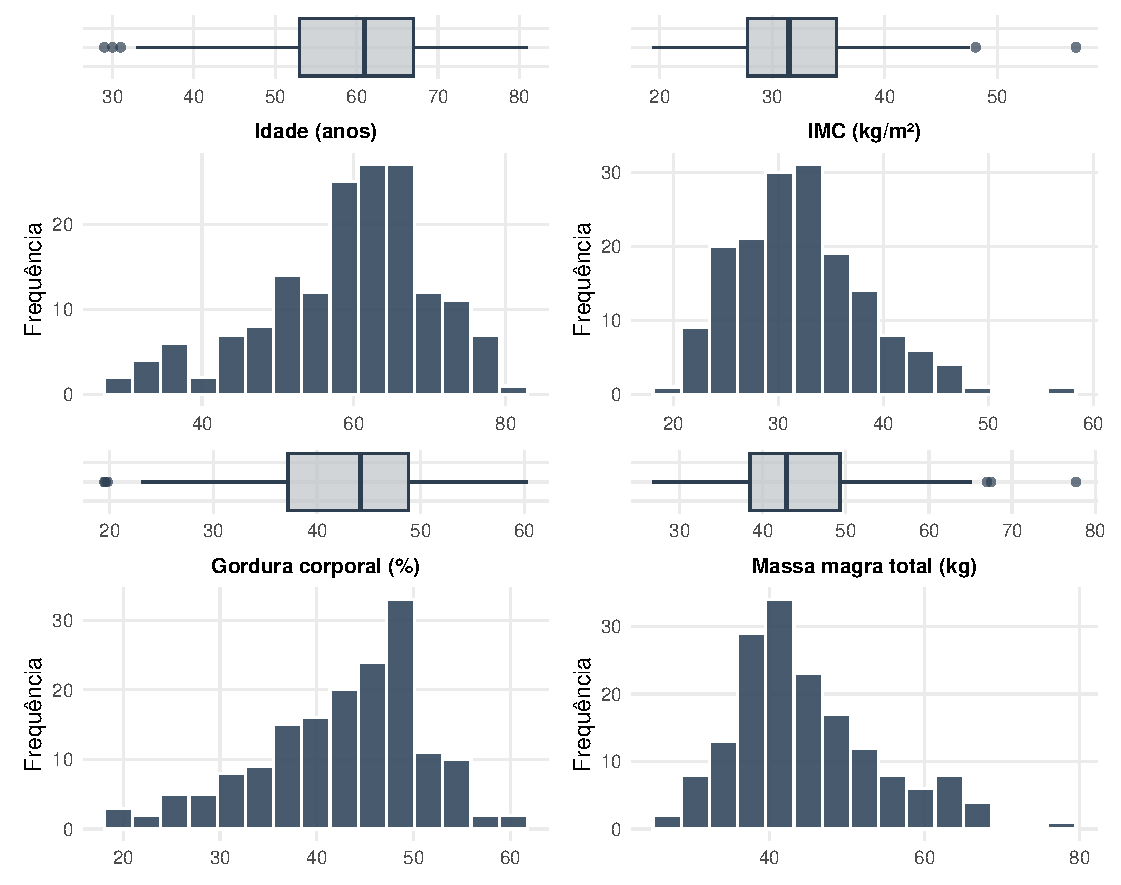
\includegraphics[width=\textwidth]{outputs/painel_numericas_principais.pdf}
  \caption{Distribuições de idade, IMC, gordura corporal e massa magra total
           (histograma com boxplot).}
  \label{fig:painel_numericas}
\end{figure}

\subsubsection{Variáveis categóricas}

A amostra foi majoritariamente feminina (\PercMulheres{}) e com predominância de
etnia branca (37,6\%), parda (32,1\%) e preta (29,7\%). O sedentarismo atingiu
67,3\% dos pacientes; 67,9\% nunca fumaram e apenas 6,7\% eram fumantes atuais.
Quanto às comorbidades, \PercObesidade{} apresentavam obesidade (IMC $\geq 30$
kg/m$^2$), \PercDiabetes{} diabetes e \PercHipertensao{} hipertensão arterial.

Em relação à doença hepática, \PercDHEM{} da amostra apresentou DHEM e
\PercFibrose{} fibrose hepática significativa. Pela variável combinada, 13,3\%
dos pacientes não têm DHEM, 61,2\% têm DHEM sem fibrose e 25,5\% têm DHEM com
fibrose.

A frequência de sarcopenia variou substancialmente conforme o critério: entre os
testes funcionais, SARC-F $\geq 4$ identificou \PercSarcSARCF{} dos avaliados,
SARC-F com panturrilha $\geq 11$ identificou \PercSarcSARCFCC{}, handgrip
\PercSarcHandgrip{}, elevação da cadeira \PercSarcElev{} e velocidade de marcha
\PercSarcVel{}. Entre os ajustes de massa magra, a frequência de baixa MMEA foi
de \PercIMMANewman{} (Newman), \PercIMMABaumgartner{} (Baumgartner),
\PercIMMAFNIH{} (FNIH) e \PercIMMAPeso{} (razão MMEA/peso); quando combinados ao
handgrip, as prevalências de sarcopenia foram \PercSarcNewman{},
\PercSarcBaumgartner{} e \PercSarcFNIH{}.

A Tabela~\ref{tab:categoricas} apresenta as frequências completas de todas as
variáveis categóricas, e a Figura~\ref{fig:painel_categoricas} ilustra as
principais.


\begin{longtable}[t]{lrl}
\caption{Frequências absolutas e relativas das variáveis categóricas. Percentuais calculados sobre os dados observados; níveis sem ocorrência aparecem com frequência zero.\label{tab:categoricas}}\\
\toprule
Característica & Freq. Absoluta & Freq. Relativa (\%)\\
\midrule
\endfirsthead
\caption[]{Frequências absolutas e relativas das variáveis categóricas. Percentuais calculados sobre os dados observados; níveis sem ocorrência aparecem com frequência zero. \textit{(continuação)}}\\
\toprule
Característica & Freq. Absoluta & Freq. Relativa (\%)\\
\midrule
\endhead

\endfoot
\bottomrule
\endlastfoot
\addlinespace[0.3em]
\multicolumn{3}{l}{\textbf{Sexo (n = 165)}}\\
\hspace{1em}\cellcolor{gray!10}{Feminino} & \cellcolor{gray!10}{132} & \cellcolor{gray!10}{80,0}\\
\hspace{1em}Masculino & 33 & 20,0\\
\addlinespace[0.3em]
\multicolumn{3}{l}{\textbf{Etnia (n = 165)}}\\
\hspace{1em}\cellcolor{gray!10}{Branca} & \cellcolor{gray!10}{62} & \cellcolor{gray!10}{37,6}\\
\hspace{1em}Preta & 49 & 29,7\\
\hspace{1em}\cellcolor{gray!10}{Parda} & \cellcolor{gray!10}{53} & \cellcolor{gray!10}{32,1}\\
\hspace{1em}Outras & 1 & 0,6\\
\addlinespace[0.3em]
\multicolumn{3}{l}{\textbf{Atividade física (n = 165)}}\\
\hspace{1em}\cellcolor{gray!10}{Sedentário} & \cellcolor{gray!10}{111} & \cellcolor{gray!10}{67,3}\\
\hspace{1em}>150 min/sem & 34 & 20,6\\
\hspace{1em}\cellcolor{gray!10}{<150 min/sem} & \cellcolor{gray!10}{20} & \cellcolor{gray!10}{12,1}\\
\addlinespace[0.3em]
\multicolumn{3}{l}{\textbf{Tabagismo (n = 165)}}\\
\hspace{1em}Nunca fumou & 112 & 67,9\\
\hspace{1em}\cellcolor{gray!10}{Fumante} & \cellcolor{gray!10}{11} & \cellcolor{gray!10}{6,7}\\
\hspace{1em}Ex-fumante & 42 & 25,5\\
\addlinespace[0.3em]
\multicolumn{3}{l}{\textbf{Obesidade (IMC $\geq$ 30 kg/m²) (n = 165)}}\\
\hspace{1em}\cellcolor{gray!10}{Não} & \cellcolor{gray!10}{62} & \cellcolor{gray!10}{37,6}\\
\hspace{1em}Sim & 103 & 62,4\\
\addlinespace[0.3em]
\multicolumn{3}{l}{\textbf{Sobrepeso (n = 165)}}\\
\hspace{1em}\cellcolor{gray!10}{Não} & \cellcolor{gray!10}{134} & \cellcolor{gray!10}{81,2}\\
\hspace{1em}Sim & 31 & 18,8\\
\addlinespace[0.3em]
\multicolumn{3}{l}{\textbf{Diabetes (n = 165)}}\\
\hspace{1em}\cellcolor{gray!10}{Não} & \cellcolor{gray!10}{44} & \cellcolor{gray!10}{26,7}\\
\hspace{1em}Sim & 121 & 73,3\\
\addlinespace[0.3em]
\multicolumn{3}{l}{\textbf{Hipertensão arterial (n = 165)}}\\
\hspace{1em}\cellcolor{gray!10}{Não} & \cellcolor{gray!10}{28} & \cellcolor{gray!10}{17,0}\\
\hspace{1em}Sim & 137 & 83,0\\
\addlinespace[0.3em]
\multicolumn{3}{l}{\textbf{DHEM (n = 165)}}\\
\hspace{1em}\cellcolor{gray!10}{Não} & \cellcolor{gray!10}{27} & \cellcolor{gray!10}{16,4}\\
\hspace{1em}Sim & 138 & 83,6\\
\addlinespace[0.3em]
\multicolumn{3}{l}{\textbf{Esteatose pelo FLI (n = 126; 39 ausentes)}}\\
\hspace{1em}\cellcolor{gray!10}{Não} & \cellcolor{gray!10}{29} & \cellcolor{gray!10}{23,0}\\
\hspace{1em}Sim & 97 & 77,0\\
\addlinespace[0.3em]
\multicolumn{3}{l}{\textbf{Esteatose (Saadeh) (n = 158; 7 ausentes)}}\\
\hspace{1em}\cellcolor{gray!10}{Não} & \cellcolor{gray!10}{22} & \cellcolor{gray!10}{13,9}\\
\hspace{1em}Sim & 136 & 86,1\\
\addlinespace[0.3em]
\multicolumn{3}{l}{\textbf{Esteatose pelo CAP (n = 165)}}\\
\hspace{1em}\cellcolor{gray!10}{Não} & \cellcolor{gray!10}{67} & \cellcolor{gray!10}{40,6}\\
\hspace{1em}Sim & 98 & 59,4\\
\addlinespace[0.3em]
\multicolumn{3}{l}{\textbf{Fibrose hepática significativa (n = 165)}}\\
\hspace{1em}\cellcolor{gray!10}{Não} & \cellcolor{gray!10}{123} & \cellcolor{gray!10}{74,5}\\
\hspace{1em}Sim & 42 & 25,5\\
\addlinespace[0.3em]
\multicolumn{3}{l}{\textbf{Grupo DHEM/fibrose (n = 165)}}\\
\hspace{1em}\cellcolor{gray!10}{Sem DHEM} & \cellcolor{gray!10}{22} & \cellcolor{gray!10}{13,3}\\
\hspace{1em}DHEM sem Fibrose & 101 & 61,2\\
\hspace{1em}\cellcolor{gray!10}{DHEM com Fibrose} & \cellcolor{gray!10}{42} & \cellcolor{gray!10}{25,5}\\
\addlinespace[0.3em]
\multicolumn{3}{l}{\textbf{Gordura corporal (n = 165)}}\\
\hspace{1em}Normal & 39 & 23,6\\
\hspace{1em}\cellcolor{gray!10}{Alta} & \cellcolor{gray!10}{126} & \cellcolor{gray!10}{76,4}\\
\addlinespace[0.3em]
\multicolumn{3}{l}{\textbf{Baixa massa magra (MMEA \textless{} 15/20 kg) (n = 165)}}\\
\hspace{1em}Normal & 140 & 84,8\\
\hspace{1em}\cellcolor{gray!10}{Reduzido} & \cellcolor{gray!10}{25} & \cellcolor{gray!10}{15,2}\\
\addlinespace[0.3em]
\multicolumn{3}{l}{\textbf{MMEA (Newman) (n = 165)}}\\
\hspace{1em}Normal & 91 & 55,2\\
\hspace{1em}\cellcolor{gray!10}{Reduzido} & \cellcolor{gray!10}{74} & \cellcolor{gray!10}{44,8}\\
\addlinespace[0.3em]
\multicolumn{3}{l}{\textbf{Sarcopenia (Newman + handgrip) (n = 165)}}\\
\hspace{1em}Não & 143 & 86,7\\
\hspace{1em}\cellcolor{gray!10}{Sim} & \cellcolor{gray!10}{22} & \cellcolor{gray!10}{13,3}\\
\addlinespace[0.3em]
\multicolumn{3}{l}{\textbf{MMEA (Baumgartner) (n = 165)}}\\
\hspace{1em}Normal & 153 & 92,7\\
\hspace{1em}\cellcolor{gray!10}{Reduzido} & \cellcolor{gray!10}{12} & \cellcolor{gray!10}{7,3}\\
\addlinespace[0.3em]
\multicolumn{3}{l}{\textbf{Sarcopenia (Baumgartner + handgrip) (n = 165)}}\\
\hspace{1em}Não & 161 & 97,6\\
\hspace{1em}\cellcolor{gray!10}{Sim} & \cellcolor{gray!10}{4} & \cellcolor{gray!10}{2,4}\\
\addlinespace[0.3em]
\multicolumn{3}{l}{\textbf{MMEA (FNIH) (n = 165)}}\\
\hspace{1em}Normal & 130 & 78,8\\
\hspace{1em}\cellcolor{gray!10}{Reduzido} & \cellcolor{gray!10}{35} & \cellcolor{gray!10}{21,2}\\
\addlinespace[0.3em]
\multicolumn{3}{l}{\textbf{Sarcopenia (FNIH + handgrip) (n = 165)}}\\
\hspace{1em}Não & 152 & 92,1\\
\hspace{1em}\cellcolor{gray!10}{Sim} & \cellcolor{gray!10}{13} & \cellcolor{gray!10}{7,9}\\
\addlinespace[0.3em]
\multicolumn{3}{l}{\textbf{MMEA (peso) (n = 165)}}\\
\hspace{1em}Normal & 152 & 92,1\\
\hspace{1em}\cellcolor{gray!10}{Reduzido} & \cellcolor{gray!10}{13} & \cellcolor{gray!10}{7,9}\\
\addlinespace[0.3em]
\multicolumn{3}{l}{\textbf{Sarcopenia (obesidade sarcopênica) (n = 165)}}\\
\hspace{1em}Não & 165 & 100,0\\
\hspace{1em}\cellcolor{gray!10}{Sim} & \cellcolor{gray!10}{0} & \cellcolor{gray!10}{0,0}\\
\addlinespace[0.3em]
\multicolumn{3}{l}{\textbf{Sarcopenia (SARC-F $\geq$ 4) (n = 150; 15 ausentes)}}\\
\hspace{1em}Normal & 109 & 72,7\\
\hspace{1em}\cellcolor{gray!10}{Alterado} & \cellcolor{gray!10}{41} & \cellcolor{gray!10}{27,3}\\
\addlinespace[0.3em]
\multicolumn{3}{l}{\textbf{Sarcopenia (SARC-F + panturrilha $\geq$ 11) (n = 148; 17 ausentes)}}\\
\hspace{1em}Normal & 119 & 80,4\\
\hspace{1em}\cellcolor{gray!10}{Alterado} & \cellcolor{gray!10}{29} & \cellcolor{gray!10}{19,6}\\
\addlinespace[0.3em]
\multicolumn{3}{l}{\textbf{Sarcopenia (handgrip \textless{} 16/27 kg) (n = 134; 31 ausentes)}}\\
\hspace{1em}Normal & 94 & 70,1\\
\hspace{1em}\cellcolor{gray!10}{Alterado} & \cellcolor{gray!10}{40} & \cellcolor{gray!10}{29,9}\\
\addlinespace[0.3em]
\multicolumn{3}{l}{\textbf{Sarcopenia (elevação da cadeira \textgreater{} 15 s) (n = 134; 31 ausentes)}}\\
\hspace{1em}Normal & 70 & 52,2\\
\hspace{1em}\cellcolor{gray!10}{Alterado} & \cellcolor{gray!10}{64} & \cellcolor{gray!10}{47,8}\\
\addlinespace[0.3em]
\multicolumn{3}{l}{\textbf{Sarcopenia (velocidade de marcha \textless{} 0,8 m/s) (n = 126; 39 ausentes)}}\\
\hspace{1em}Normal & 28 & 22,2\\
\hspace{1em}\cellcolor{gray!10}{Alterado} & \cellcolor{gray!10}{98} & \cellcolor{gray!10}{77,8}\\*
\end{longtable}


\begin{figure}[H]
  \centering
  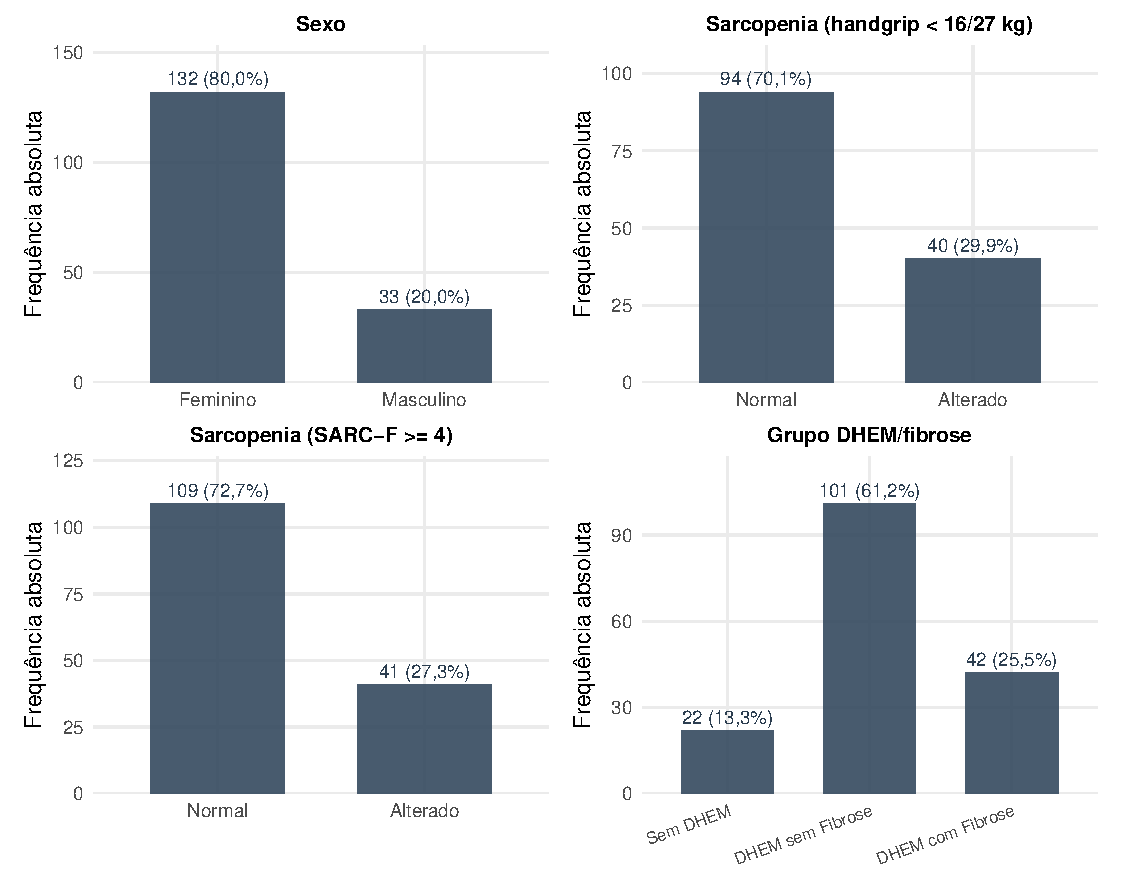
\includegraphics[width=\textwidth]{outputs/painel_categoricas_principais.pdf}
  \caption{Distribuição de sexo, grupo DHEM/fibrose e sarcopenia pelos critérios
           de handgrip e SARC-F (frequências absolutas e relativas).}
  \label{fig:painel_categoricas}
\end{figure}

\subsection{Análise Descritiva Bivariada}

\subsubsection{Caracterização segundo o grupo DHEM/fibrose}

A Tabela~\ref{tab:cruzamento} resume as características da amostra segundo os
grupos sem DHEM ($n = \NSemDHEM$), DHEM sem fibrose ($n = \NDHEMSemFibrose$) e
DHEM com fibrose ($n = \NDHEMComFibrose$).

Observa-se um gradiente crescente de obesidade e adiposidade com a gravidade da
doença hepática: a obesidade passou de 40,9\% (sem DHEM) para 61,4\% (DHEM sem
fibrose) e 76,2\% (DHEM com fibrose); o IMC médio passou de 29,2 para 32,1 e
34,0 kg/m$^2$, e a gordura corporal de 38,9\% para 42,4\% e 45,2\%. A massa
magra total, por sua vez, foi semelhante entre os grupos (43,0, 45,0 e 45,1 kg),
bem como a idade (62,0, 58,0 e 60,5 anos). As razões de massa magra ajustadas
pelo peso (MMEA/peso: 26,5, 24,7 e 23,2) e pelo IMC (MMEA/IMC: 0,7, 0,6 e 0,6)
apresentaram valores decrescentes com a gravidade, sugerindo menor massa magra
relativa nos grupos mais graves.

\begingroup\fontsize{9}{11}\selectfont\setlength{\tabcolsep}{3pt}

\begin{longtable}[t]{>{\raggedright\arraybackslash}p{4.3cm}>{\raggedright\arraybackslash}p{2.6cm}>{\raggedright\arraybackslash}p{2.6cm}>{\raggedright\arraybackslash}p{2.6cm}>{\raggedright\arraybackslash}p{2.6cm}}
\caption{Características clínicas, demográficas e de composição corporal segundo o grupo DHEM/fibrose. Percentuais calculados sobre os dados observados.\label{tab:cruzamento}}\\
\toprule
Característica / Métrica & Geral (n = 165) & Sem DHEM (n = 22) & DHEM sem Fibrose (n = 101) & DHEM com Fibrose (n = 42)\\
\midrule
\endfirsthead
\caption[]{Características clínicas, demográficas e de composição corporal segundo o grupo DHEM/fibrose. Percentuais calculados sobre os dados observados. \textit{(continuação)}}\\
\toprule
Característica / Métrica & Geral (n = 165) & Sem DHEM (n = 22) & DHEM sem Fibrose (n = 101) & DHEM com Fibrose (n = 42)\\
\midrule
\endhead

\endfoot
\bottomrule
\endlastfoot
\addlinespace[0.3em]
\multicolumn{5}{l}{\textbf{Características sociodemográficas}}\\
\addlinespace[0.3em]
\multicolumn{5}{l}{\textbf{Sexo}}\\
\hspace{1em}\hspace{1em}\cellcolor{gray!10}{Feminino} & \cellcolor{gray!10}{132 (80,0\%)} & \cellcolor{gray!10}{17 (77,3\%)} & \cellcolor{gray!10}{78 (77,2\%)} & \cellcolor{gray!10}{37 (88,1\%)}\\
\hspace{1em}\hspace{1em}Masculino & 33 (20,0\%) & 5 (22,7\%) & 23 (22,8\%) & 5 (11,9\%)\\
\addlinespace[0.3em]
\multicolumn{5}{l}{\textbf{Etnia}}\\
\hspace{1em}\hspace{1em}\cellcolor{gray!10}{Branca} & \cellcolor{gray!10}{62 (37,6\%)} & \cellcolor{gray!10}{5 (22,7\%)} & \cellcolor{gray!10}{35 (34,7\%)} & \cellcolor{gray!10}{22 (52,4\%)}\\
\hspace{1em}\hspace{1em}Preta & 49 (29,7\%) & 10 (45,5\%) & 32 (31,7\%) & 7 (16,7\%)\\
\hspace{1em}\hspace{1em}\cellcolor{gray!10}{Parda} & \cellcolor{gray!10}{53 (32,1\%)} & \cellcolor{gray!10}{7 (31,8\%)} & \cellcolor{gray!10}{34 (33,7\%)} & \cellcolor{gray!10}{12 (28,6\%)}\\
\hspace{1em}\hspace{1em}Outras & 1 (0,6\%) & 0 (0,0\%) & 0 (0,0\%) & 1 (2,4\%)\\
\addlinespace[0.3em]
\multicolumn{5}{l}{\textbf{Atividade física}}\\
\hspace{1em}\hspace{1em}\cellcolor{gray!10}{Sedentário} & \cellcolor{gray!10}{111 (67,3\%)} & \cellcolor{gray!10}{10 (45,5\%)} & \cellcolor{gray!10}{68 (67,3\%)} & \cellcolor{gray!10}{33 (78,6\%)}\\
\hspace{1em}\hspace{1em}\textgreater{}150 min/sem & 34 (20,6\%) & 9 (40,9\%) & 19 (18,8\%) & 6 (14,3\%)\\
\hspace{1em}\hspace{1em}\cellcolor{gray!10}{\textless{}150 min/sem} & \cellcolor{gray!10}{20 (12,1\%)} & \cellcolor{gray!10}{3 (13,6\%)} & \cellcolor{gray!10}{14 (13,9\%)} & \cellcolor{gray!10}{3 (7,1\%)}\\
\addlinespace[0.3em]
\multicolumn{5}{l}{\textbf{Tabagismo}}\\
\hspace{1em}\hspace{1em}Nunca fumou & 112 (67,9\%) & 15 (68,2\%) & 72 (71,3\%) & 25 (59,5\%)\\
\hspace{1em}\hspace{1em}\cellcolor{gray!10}{Fumante} & \cellcolor{gray!10}{11 (6,7\%)} & \cellcolor{gray!10}{1 (4,5\%)} & \cellcolor{gray!10}{7 (6,9\%)} & \cellcolor{gray!10}{3 (7,1\%)}\\
\hspace{1em}\hspace{1em}Ex-fumante & 42 (25,5\%) & 6 (27,3\%) & 22 (21,8\%) & 14 (33,3\%)\\
\addlinespace[0.3em]
\multicolumn{5}{l}{\textbf{Comorbidades}}\\
\addlinespace[0.3em]
\multicolumn{5}{l}{\textbf{Obesidade (IMC $\geq$ 30 kg/m²)}}\\
\hspace{1em}\hspace{1em}\cellcolor{gray!10}{Não} & \cellcolor{gray!10}{62 (37,6\%)} & \cellcolor{gray!10}{13 (59,1\%)} & \cellcolor{gray!10}{39 (38,6\%)} & \cellcolor{gray!10}{10 (23,8\%)}\\
\hspace{1em}\hspace{1em}Sim & 103 (62,4\%) & 9 (40,9\%) & 62 (61,4\%) & 32 (76,2\%)\\
\addlinespace[0.3em]
\multicolumn{5}{l}{\textbf{Sobrepeso}}\\
\hspace{1em}\hspace{1em}\cellcolor{gray!10}{Não} & \cellcolor{gray!10}{134 (81,2\%)} & \cellcolor{gray!10}{19 (86,4\%)} & \cellcolor{gray!10}{78 (77,2\%)} & \cellcolor{gray!10}{37 (88,1\%)}\\
\hspace{1em}\hspace{1em}Sim & 31 (18,8\%) & 3 (13,6\%) & 23 (22,8\%) & 5 (11,9\%)\\
\addlinespace[0.3em]
\multicolumn{5}{l}{\textbf{Diabetes}}\\
\hspace{1em}\hspace{1em}\cellcolor{gray!10}{Não} & \cellcolor{gray!10}{44 (26,7\%)} & \cellcolor{gray!10}{8 (36,4\%)} & \cellcolor{gray!10}{27 (26,7\%)} & \cellcolor{gray!10}{9 (21,4\%)}\\
\hspace{1em}\hspace{1em}Sim & 121 (73,3\%) & 14 (63,6\%) & 74 (73,3\%) & 33 (78,6\%)\\
\addlinespace[0.3em]
\multicolumn{5}{l}{\textbf{Hipertensão arterial}}\\
\hspace{1em}\hspace{1em}\cellcolor{gray!10}{Não} & \cellcolor{gray!10}{28 (17,0\%)} & \cellcolor{gray!10}{3 (13,6\%)} & \cellcolor{gray!10}{18 (17,8\%)} & \cellcolor{gray!10}{7 (16,7\%)}\\
\hspace{1em}\hspace{1em}Sim & 137 (83,0\%) & 19 (86,4\%) & 83 (82,2\%) & 35 (83,3\%)\\
\addlinespace[0.3em]
\multicolumn{5}{l}{\textbf{Doença hepática}}\\
\addlinespace[0.3em]
\multicolumn{5}{l}{\textbf{DHEM}}\\
\hspace{1em}\hspace{1em}\cellcolor{gray!10}{Não} & \cellcolor{gray!10}{27 (16,4\%)} & \cellcolor{gray!10}{22 (100,0\%)} & \cellcolor{gray!10}{0 (0,0\%)} & \cellcolor{gray!10}{5 (11,9\%)}\\
\hspace{1em}\hspace{1em}Sim & 138 (83,6\%) & 0 (0,0\%) & 101 (100,0\%) & 37 (88,1\%)\\
\addlinespace[0.3em]
\multicolumn{5}{l}{\textbf{Esteatose pelo FLI}}\\
\hspace{1em}\hspace{1em}\cellcolor{gray!10}{Não} & \cellcolor{gray!10}{29 (23,0\%)} & \cellcolor{gray!10}{0 (0,0\%)} & \cellcolor{gray!10}{26 (28,9\%)} & \cellcolor{gray!10}{3 (8,3\%)}\\
\hspace{1em}\hspace{1em}Sim & 97 (77,0\%) & 0 (0,0\%) & 64 (71,1\%) & 33 (91,7\%)\\
\addlinespace[0.3em]
\multicolumn{5}{l}{\textbf{Esteatose (Saadeh)}}\\
\hspace{1em}\hspace{1em}\cellcolor{gray!10}{Não} & \cellcolor{gray!10}{22 (13,9\%)} & \cellcolor{gray!10}{17 (100,0\%)} & \cellcolor{gray!10}{1 (1,0\%)} & \cellcolor{gray!10}{4 (9,8\%)}\\
\hspace{1em}\hspace{1em}Sim & 136 (86,1\%) & 0 (0,0\%) & 99 (99,0\%) & 37 (90,2\%)\\
\addlinespace[0.3em]
\multicolumn{5}{l}{\textbf{Esteatose pelo CAP}}\\
\hspace{1em}\hspace{1em}\cellcolor{gray!10}{Não} & \cellcolor{gray!10}{67 (40,6\%)} & \cellcolor{gray!10}{22 (100,0\%)} & \cellcolor{gray!10}{32 (31,7\%)} & \cellcolor{gray!10}{13 (31,0\%)}\\
\hspace{1em}\hspace{1em}Sim & 98 (59,4\%) & 0 (0,0\%) & 69 (68,3\%) & 29 (69,0\%)\\
\addlinespace[0.3em]
\multicolumn{5}{l}{\textbf{Composição corporal e sarcopenia}}\\
\addlinespace[0.3em]
\multicolumn{5}{l}{\textbf{Gordura corporal}}\\
\hspace{1em}\hspace{1em}\cellcolor{gray!10}{Normal} & \cellcolor{gray!10}{39 (23,6\%)} & \cellcolor{gray!10}{9 (40,9\%)} & \cellcolor{gray!10}{23 (22,8\%)} & \cellcolor{gray!10}{7 (16,7\%)}\\
\hspace{1em}\hspace{1em}Alta & 126 (76,4\%) & 13 (59,1\%) & 78 (77,2\%) & 35 (83,3\%)\\
\addlinespace[0.3em]
\multicolumn{5}{l}{\textbf{Baixa massa magra (MMEA \textless{} 15/20 kg)}}\\
\hspace{1em}\hspace{1em}\cellcolor{gray!10}{Normal} & \cellcolor{gray!10}{140 (84,8\%)} & \cellcolor{gray!10}{19 (86,4\%)} & \cellcolor{gray!10}{84 (83,2\%)} & \cellcolor{gray!10}{37 (88,1\%)}\\
\hspace{1em}\hspace{1em}Reduzido & 25 (15,2\%) & 3 (13,6\%) & 17 (16,8\%) & 5 (11,9\%)\\
\addlinespace[0.3em]
\multicolumn{5}{l}{\textbf{MMEA (Newman)}}\\
\hspace{1em}\hspace{1em}\cellcolor{gray!10}{Normal} & \cellcolor{gray!10}{91 (55,2\%)} & \cellcolor{gray!10}{12 (54,5\%)} & \cellcolor{gray!10}{59 (58,4\%)} & \cellcolor{gray!10}{20 (47,6\%)}\\
\hspace{1em}\hspace{1em}Reduzido & 74 (44,8\%) & 10 (45,5\%) & 42 (41,6\%) & 22 (52,4\%)\\
\addlinespace[0.3em]
\multicolumn{5}{l}{\textbf{Sarcopenia (Newman + handgrip)}}\\
\hspace{1em}\hspace{1em}\cellcolor{gray!10}{Não} & \cellcolor{gray!10}{143 (86,7\%)} & \cellcolor{gray!10}{18 (81,8\%)} & \cellcolor{gray!10}{88 (87,1\%)} & \cellcolor{gray!10}{37 (88,1\%)}\\
\hspace{1em}\hspace{1em}Sim & 22 (13,3\%) & 4 (18,2\%) & 13 (12,9\%) & 5 (11,9\%)\\
\addlinespace[0.3em]
\multicolumn{5}{l}{\textbf{MMEA (Baumgartner)}}\\
\hspace{1em}\hspace{1em}\cellcolor{gray!10}{Normal} & \cellcolor{gray!10}{153 (92,7\%)} & \cellcolor{gray!10}{21 (95,5\%)} & \cellcolor{gray!10}{93 (92,1\%)} & \cellcolor{gray!10}{39 (92,9\%)}\\
\hspace{1em}\hspace{1em}Reduzido & 12 (7,3\%) & 1 (4,5\%) & 8 (7,9\%) & 3 (7,1\%)\\
\addlinespace[0.3em]
\multicolumn{5}{l}{\textbf{Sarcopenia (Baumgartner + handgrip)}}\\
\hspace{1em}\hspace{1em}\cellcolor{gray!10}{Não} & \cellcolor{gray!10}{161 (97,6\%)} & \cellcolor{gray!10}{22 (100,0\%)} & \cellcolor{gray!10}{97 (96,0\%)} & \cellcolor{gray!10}{42 (100,0\%)}\\
\hspace{1em}\hspace{1em}Sim & 4 (2,4\%) & 0 (0,0\%) & 4 (4,0\%) & 0 (0,0\%)\\
\addlinespace[0.3em]
\multicolumn{5}{l}{\textbf{MMEA (FNIH)}}\\
\hspace{1em}\hspace{1em}\cellcolor{gray!10}{Normal} & \cellcolor{gray!10}{130 (78,8\%)} & \cellcolor{gray!10}{20 (90,9\%)} & \cellcolor{gray!10}{80 (79,2\%)} & \cellcolor{gray!10}{30 (71,4\%)}\\
\hspace{1em}\hspace{1em}Reduzido & 35 (21,2\%) & 2 (9,1\%) & 21 (20,8\%) & 12 (28,6\%)\\
\addlinespace[0.3em]
\multicolumn{5}{l}{\textbf{Sarcopenia (FNIH + handgrip)}}\\
\hspace{1em}\hspace{1em}\cellcolor{gray!10}{Não} & \cellcolor{gray!10}{152 (92,1\%)} & \cellcolor{gray!10}{21 (95,5\%)} & \cellcolor{gray!10}{93 (92,1\%)} & \cellcolor{gray!10}{38 (90,5\%)}\\
\hspace{1em}\hspace{1em}Sim & 13 (7,9\%) & 1 (4,5\%) & 8 (7,9\%) & 4 (9,5\%)\\
\addlinespace[0.3em]
\multicolumn{5}{l}{\textbf{MMEA (peso)}}\\
\hspace{1em}\hspace{1em}\cellcolor{gray!10}{Normal} & \cellcolor{gray!10}{152 (92,1\%)} & \cellcolor{gray!10}{22 (100,0\%)} & \cellcolor{gray!10}{93 (92,1\%)} & \cellcolor{gray!10}{37 (88,1\%)}\\
\hspace{1em}\hspace{1em}Reduzido & 13 (7,9\%) & 0 (0,0\%) & 8 (7,9\%) & 5 (11,9\%)\\
\addlinespace[0.3em]
\multicolumn{5}{l}{\textbf{Sarcopenia (obesidade sarcopênica)}}\\
\hspace{1em}\hspace{1em}\cellcolor{gray!10}{Não} & \cellcolor{gray!10}{165 (100,0\%)} & \cellcolor{gray!10}{22 (100,0\%)} & \cellcolor{gray!10}{101 (100,0\%)} & \cellcolor{gray!10}{42 (100,0\%)}\\
\hspace{1em}\hspace{1em}Sim & 0 (0,0\%) & 0 (0,0\%) & 0 (0,0\%) & 0 (0,0\%)\\
\addlinespace[0.3em]
\multicolumn{5}{l}{\textbf{Sarcopenia (SARC-F $\geq$ 4)}}\\
\hspace{1em}\hspace{1em}\cellcolor{gray!10}{Normal} & \cellcolor{gray!10}{109 (72,7\%)} & \cellcolor{gray!10}{17 (85,0\%)} & \cellcolor{gray!10}{66 (74,2\%)} & \cellcolor{gray!10}{26 (63,4\%)}\\
\hspace{1em}\hspace{1em}Alterado & 41 (27,3\%) & 3 (15,0\%) & 23 (25,8\%) & 15 (36,6\%)\\
\addlinespace[0.3em]
\multicolumn{5}{l}{\textbf{Sarcopenia (SARC-F + panturrilha $\geq$ 11)}}\\
\hspace{1em}\hspace{1em}\cellcolor{gray!10}{Normal} & \cellcolor{gray!10}{119 (80,4\%)} & \cellcolor{gray!10}{15 (75,0\%)} & \cellcolor{gray!10}{71 (81,6\%)} & \cellcolor{gray!10}{33 (80,5\%)}\\
\hspace{1em}\hspace{1em}Alterado & 29 (19,6\%) & 5 (25,0\%) & 16 (18,4\%) & 8 (19,5\%)\\
\addlinespace[0.3em]
\multicolumn{5}{l}{\textbf{Sarcopenia (handgrip \textless{} 16/27 kg)}}\\
\hspace{1em}\hspace{1em}\cellcolor{gray!10}{Normal} & \cellcolor{gray!10}{94 (70,1\%)} & \cellcolor{gray!10}{13 (68,4\%)} & \cellcolor{gray!10}{53 (67,9\%)} & \cellcolor{gray!10}{28 (75,7\%)}\\
\hspace{1em}\hspace{1em}Alterado & 40 (29,9\%) & 6 (31,6\%) & 25 (32,1\%) & 9 (24,3\%)\\
\addlinespace[0.3em]
\multicolumn{5}{l}{\textbf{Sarcopenia (elevação da cadeira \textgreater{} 15 s)}}\\
\hspace{1em}\hspace{1em}\cellcolor{gray!10}{Normal} & \cellcolor{gray!10}{70 (52,2\%)} & \cellcolor{gray!10}{13 (68,4\%)} & \cellcolor{gray!10}{44 (55,0\%)} & \cellcolor{gray!10}{13 (37,1\%)}\\
\hspace{1em}\hspace{1em}Alterado & 64 (47,8\%) & 6 (31,6\%) & 36 (45,0\%) & 22 (62,9\%)\\
\addlinespace[0.3em]
\multicolumn{5}{l}{\textbf{Sarcopenia (velocidade de marcha \textless{} 0,8 m/s)}}\\
\hspace{1em}\hspace{1em}\cellcolor{gray!10}{Normal} & \cellcolor{gray!10}{28 (22,2\%)} & \cellcolor{gray!10}{8 (42,1\%)} & \cellcolor{gray!10}{14 (18,4\%)} & \cellcolor{gray!10}{6 (19,4\%)}\\
\hspace{1em}\hspace{1em}Alterado & 98 (77,8\%) & 11 (57,9\%) & 62 (81,6\%) & 25 (80,6\%)\\
\addlinespace[0.3em]
\multicolumn{5}{l}{\textbf{Variáveis numéricas}}\\
\addlinespace[0.3em]
\multicolumn{5}{l}{\textbf{Idade (anos)}}\\
\hspace{1em}\hspace{1em}\cellcolor{gray!10}{Média (DP)} & \cellcolor{gray!10}{59,2 (11,1)} & \cellcolor{gray!10}{62,0 (9,3)} & \cellcolor{gray!10}{58,0 (11,5)} & \cellcolor{gray!10}{60,5 (10,6)}\\
\hspace{1em}\hspace{1em}Mediana (Q1;Q3) & 61,0 (53,0;67,0) & 62,0 (58,0;68,5) & 60,0 (52,0;65,0) & 64,0 (55,2;68,5)\\
\addlinespace[0.3em]
\multicolumn{5}{l}{\textbf{Gordura corporal (\%)}}\\
\hspace{1em}\hspace{1em}\cellcolor{gray!10}{Média (DP)} & \cellcolor{gray!10}{42,7 (8,5)} & \cellcolor{gray!10}{38,9 (10,5)} & \cellcolor{gray!10}{42,4 (7,8)} & \cellcolor{gray!10}{45,2 (8,4)}\\
\hspace{1em}\hspace{1em}Mediana (Q1;Q3) & 44,2 (37,2;48,8) & 40,6 (32,6;46,9) & 43,5 (37,1;48,7) & 46,4 (41,2;49,2)\\
\addlinespace[0.3em]
\multicolumn{5}{l}{\textbf{Massa magra total (kg)}}\\
\hspace{1em}\hspace{1em}\cellcolor{gray!10}{Média (DP)} & \cellcolor{gray!10}{44,8 (9,3)} & \cellcolor{gray!10}{43,0 (9,1)} & \cellcolor{gray!10}{45,0 (9,5)} & \cellcolor{gray!10}{45,1 (9,0)}\\
\hspace{1em}\hspace{1em}Mediana (Q1;Q3) & 42,9 (38,5;49,3) & 41,2 (37,3;44,6) & 42,8 (38,6;48,9) & 43,9 (38,8;50,4)\\
\addlinespace[0.3em]
\multicolumn{5}{l}{\textbf{ALM/MMEA (kg)}}\\
\hspace{1em}\hspace{1em}\cellcolor{gray!10}{Média (DP)} & \cellcolor{gray!10}{20,0 (5,2)} & \cellcolor{gray!10}{19,6 (5,1)} & \cellcolor{gray!10}{20,1 (5,5)} & \cellcolor{gray!10}{19,8 (4,8)}\\
\hspace{1em}\hspace{1em}Mediana (Q1;Q3) & 19,1 (16,7;23,0) & 18,2 (16,7;20,7) & 19,2 (16,5;23,2) & 19,2 (16,8;23,0)\\
\addlinespace[0.3em]
\multicolumn{5}{l}{\textbf{MMEA ajustado}}\\
\hspace{1em}\hspace{1em}\cellcolor{gray!10}{Média (DP)} & \cellcolor{gray!10}{20,4 (3,3)} & \cellcolor{gray!10}{19,2 (2,6)} & \cellcolor{gray!10}{20,5 (3,3)} & \cellcolor{gray!10}{20,8 (3,3)}\\
\hspace{1em}\hspace{1em}Mediana (Q1;Q3) & 20,1 (18,1;22,0) & 18,5 (17,4;21,7) & 20,1 (18,2;21,8) & 20,5 (18,7;22,4)\\
\addlinespace[0.3em]
\multicolumn{5}{l}{\textbf{Resíduo de Newman}}\\
\hspace{1em}\hspace{1em}\cellcolor{gray!10}{Média (DP)} & \cellcolor{gray!10}{-0,4 (3,7)} & \cellcolor{gray!10}{0,4 (3,7)} & \cellcolor{gray!10}{-0,3 (3,9)} & \cellcolor{gray!10}{-1,0 (3,2)}\\
\hspace{1em}\hspace{1em}Mediana (Q1;Q3) & -1,0 (-2,7;1,5) & -1,2 (-2,0;1,6) & -0,9 (-2,6;1,5) & -1,7 (-3,0;0,7)\\
\addlinespace[0.3em]
\multicolumn{5}{l}{\textbf{MMEA/altura² (kg/m²)}}\\
\hspace{1em}\hspace{1em}\cellcolor{gray!10}{Média (DP)} & \cellcolor{gray!10}{7,8 (1,5)} & \cellcolor{gray!10}{7,6 (1,3)} & \cellcolor{gray!10}{7,9 (1,5)} & \cellcolor{gray!10}{7,8 (1,4)}\\
\hspace{1em}\hspace{1em}Mediana (Q1;Q3) & 7,6 (7,0;8,7) & 7,3 (7,1;8,2) & 7,8 (6,8;8,8) & 7,6 (7,0;8,7)\\
\addlinespace[0.3em]
\multicolumn{5}{l}{\textbf{MMEA/IMC}}\\
\hspace{1em}\hspace{1em}\cellcolor{gray!10}{Média (DP)} & \cellcolor{gray!10}{0,6 (0,2)} & \cellcolor{gray!10}{0,7 (0,2)} & \cellcolor{gray!10}{0,6 (0,2)} & \cellcolor{gray!10}{0,6 (0,1)}\\
\hspace{1em}\hspace{1em}Mediana (Q1;Q3) & 0,6 (0,5;0,7) & 0,6 (0,5;0,7) & 0,6 (0,5;0,7) & 0,6 (0,5;0,6)\\
\addlinespace[0.3em]
\multicolumn{5}{l}{\textbf{MMEA/peso}}\\
\hspace{1em}\hspace{1em}\cellcolor{gray!10}{Média (DP)} & \cellcolor{gray!10}{24,6 (4,5)} & \cellcolor{gray!10}{26,5 (5,0)} & \cellcolor{gray!10}{24,7 (4,5)} & \cellcolor{gray!10}{23,2 (3,7)}\\
\hspace{1em}\hspace{1em}Mediana (Q1;Q3) & 23,7 (21,9;26,6) & 24,6 (23,2;29,7) & 23,7 (22,3;26,8) & 23,2 (20,8;24,6)\\
\addlinespace[0.3em]
\multicolumn{5}{l}{\textbf{IMC (kg/m²)}}\\
\hspace{1em}\hspace{1em}\cellcolor{gray!10}{Média (DP)} & \cellcolor{gray!10}{32,2 (6,3)} & \cellcolor{gray!10}{29,2 (4,8)} & \cellcolor{gray!10}{32,1 (6,3)} & \cellcolor{gray!10}{34,0 (6,6)}\\
\hspace{1em}\hspace{1em}Mediana (Q1;Q3) & 31,5 (27,8;35,7) & 27,8 (25,5;32,9) & 31,4 (28,0;34,9) & 33,5 (30,4;38,6)\\*
\end{longtable}
\endgroup{}


\begin{center}
  \footnotesize
  Nota: valores expressos em $n$ (\%); percentuais calculados sobre os dados
  observados. Para variáveis com dados ausentes, o número de ausentes consta na
  Tabela~\ref{tab:categoricas}. A variável DHEM define parcialmente os grupos de
  estratificação e deve ser interpretada com cautela.
\end{center}

\subsubsection{Sarcopenia e grupos DHEM/fibrose}

Os critérios funcionais de sarcopenia apresentaram padrões distintos entre os
grupos (Figura~\ref{fig:sarc_func}). A elevação da cadeira foi o teste com
gradiente mais evidente: 31,6\% de alterados no grupo sem DHEM, 45,0\% no grupo
com DHEM sem fibrose e 62,9\% no grupo com DHEM e fibrose. Padrão semelhante foi
observado no SARC-F (15,0\%, 25,8\% e 36,6\%) e na velocidade de marcha (57,9\%,
81,6\% e 80,6\%). Já o handgrip e o SARC-F com panturrilha não mostraram
gradiente claro (prevalências entre 24\% e 32\% nos três grupos).

Entre os critérios baseados em massa magra (Figura~\ref{fig:sarc_massa}), a
prevalência de sarcopenia combinada (IMMA + handgrip) foi de 18,2\% (Newman),
0,0\% (Baumgartner) e 4,5\% (FNIH) no grupo sem DHEM; 12,9\%, 4,0\% e 7,9\% no
grupo DHEM sem fibrose; e 11,9\%, 0,0\% e 9,5\% no grupo com DHEM e fibrose —
sem um gradiente consistente de maior sarcopenia com a fibrose por esses
critérios.

\begin{figure}[H]
  \centering
  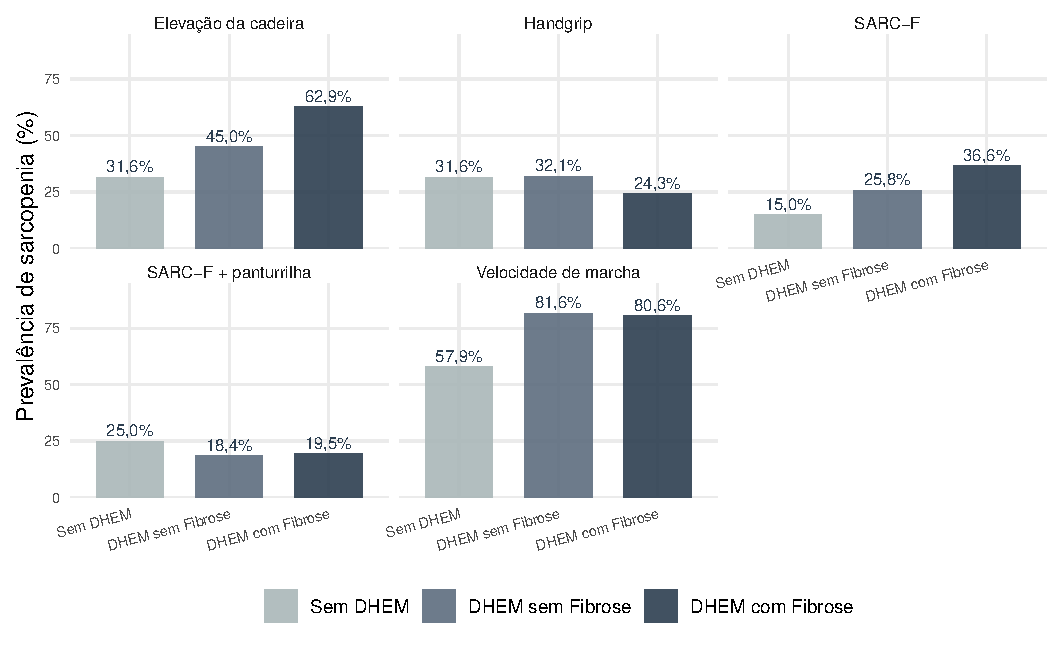
\includegraphics[width=\textwidth]{outputs/cruzamento_sarcopenia_funcional_DHEMComb.pdf}
  \caption{Prevalência de sarcopenia pelos critérios funcionais segundo o grupo
           DHEM/fibrose.}
  \label{fig:sarc_func}
\end{figure}

\begin{figure}[H]
  \centering
  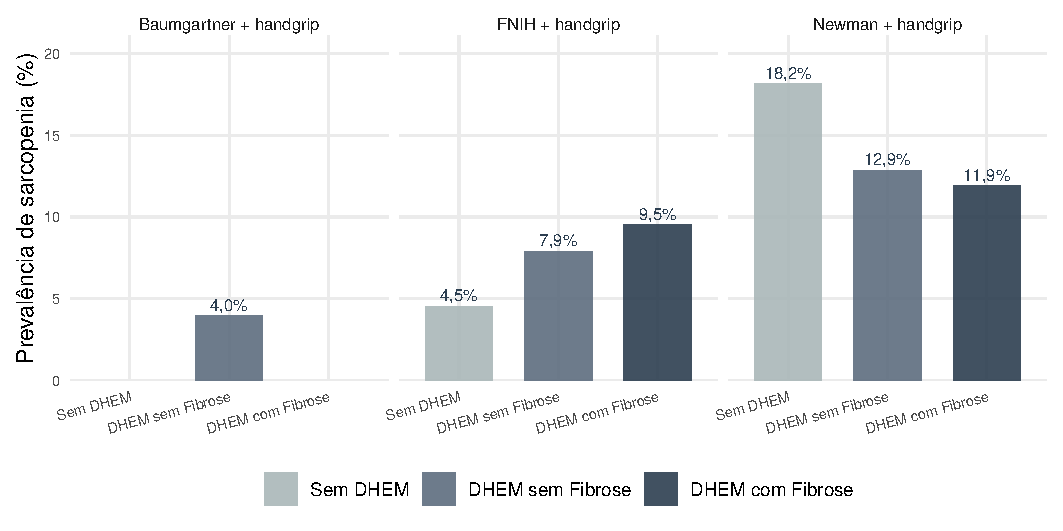
\includegraphics[width=\textwidth]{outputs/cruzamento_sarcopenia_massa_DHEMComb.pdf}
  \caption{Prevalência de sarcopenia pelos critérios de massa magra (IMMA
           ajustado + handgrip) segundo o grupo DHEM/fibrose.}
  \label{fig:sarc_massa}
\end{figure}

\subsubsection{Composição corporal e variáveis contínuas}

A Figura~\ref{fig:box_grupos} compara massa magra total e IMC entre os grupos.
Apesar da massa magra absoluta semelhante, o IMC e a gordura corporal
aumentaram com a gravidade da doença hepática, consistente com o gradiente de
obesidade descrito anteriormente.

\begin{figure}[H]
  \centering
  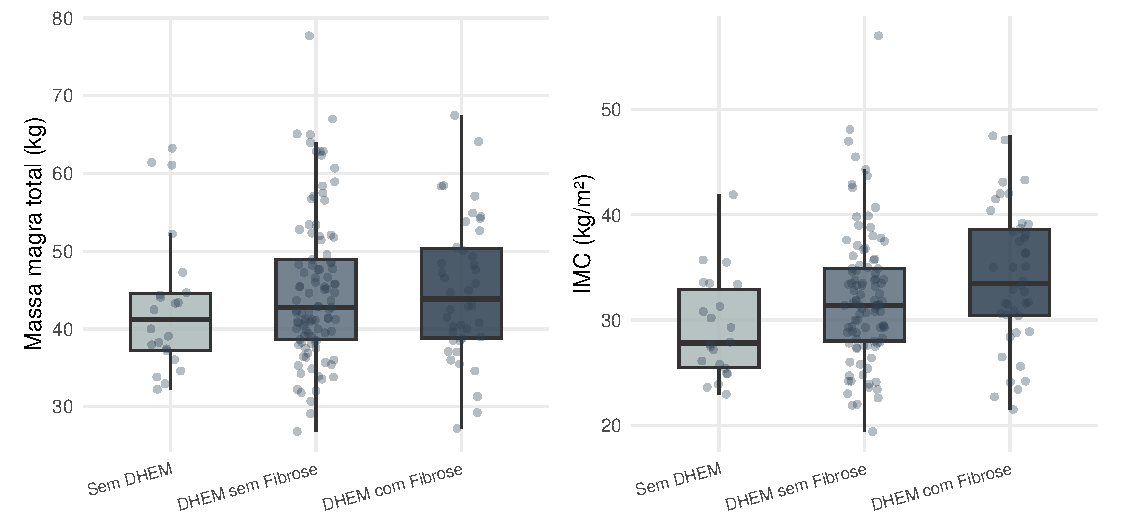
\includegraphics[width=\textwidth]{outputs/painel_boxplots_DHEMComb.pdf}
  \caption{Distribuição de massa magra total e IMC segundo o grupo DHEM/fibrose.}
  \label{fig:box_grupos}
\end{figure}

\subsubsection{Relações entre variáveis numéricas}
\label{sec:relacoes}

A matriz de correlação de Pearson (Figura~\ref{fig:correlacao}) resume as
relações lineares entre as variáveis numéricas. Destacam-se a forte correlação
entre massa magra total e ALM/MMEA ($r = 0{,}93$), as correlações moderadas
entre gordura corporal e IMC ($r = 0{,}68$) e entre massa magra e IMC
($r = 0{,}40$), e as correlações negativas entre idade e massa magra
($r = -0{,}37$) e entre as razões MMEA/IMC e MMEA/peso e o IMC ($r = -0{,}31$ e
$-0{,}40$, respectivamente).

\begin{figure}[H]
  \centering
  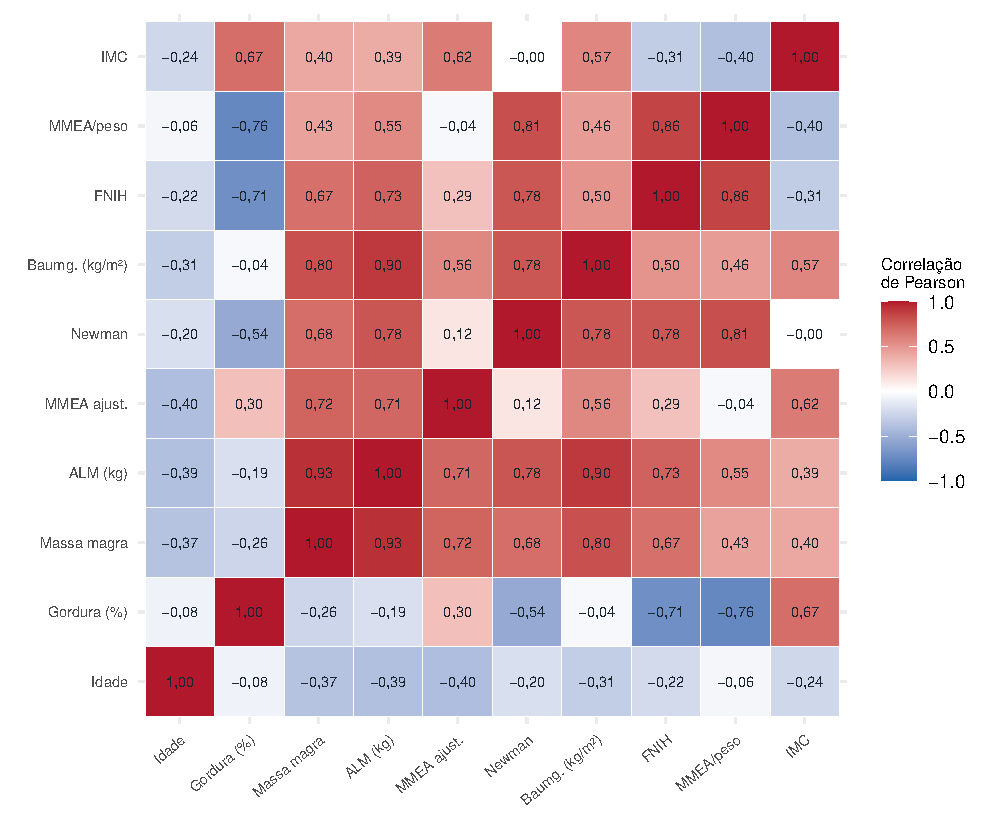
\includegraphics[width=\textwidth]{outputs/correlacao_numericas.pdf}
  \caption{Matriz de correlação de Pearson entre as variáveis numéricas.}
  \label{fig:correlacao}
\end{figure}

% ==============================================================================
\subsection{Objetivo 1: prevalência de baixa massa magra}
\label{sec:obj1}
% ==============================================================================

A Tabela~\ref{tab:prevalencia_ic} e a Figura~\ref{fig:prevalencia} apresentam a
frequência de baixa massa magra em cada critério, com IC de 95\% (método de
Wilson). A prevalência variou de 7,3\% (Baumgartner) a 44,8\% (Newman):
\PercIMMABaixo{} para o critério bruto MMEA $< 15/20$ kg
(IC 95\%: \ICIMMABaixoInf{}--\ICIMMABaixoSup{}), \PercIMMANewman{} para Newman
(IC 95\%: \ICIMMANewmanInf{}--\ICIMMANewmanSup{}), \PercIMMABaumgartner{} para
Baumgartner (IC 95\%: \ICIMMABaumgartnerInf{}--\ICIMMABaumgartnerSup{}),
\PercIMMAFNIH{} para FNIH (IC 95\%: \ICIMMAFNIHInf{}--\ICIMMAFNIHSup{}) e
\PercIMMAPeso{} para a razão MMEA/peso
(IC 95\%: \ICIMMAPesoInf{}--\ICIMMAPesoSup{}).

Para interpretar os intervalos, tomando o critério de Newman como exemplo,
estima-se que 44,8\% dos pacientes tenham baixa massa magra; se o estudo fosse
repetido muitas vezes na mesma população, em 95 de cada 100 repetições o
intervalo entre \ICIMMANewmanInf{} e \ICIMMANewmanSup{} conteria a verdadeira
prevalência. Na prática, a prevalência provável está entre aproximadamente
\ICIMMANewmanInf{} e \ICIMMANewmanSup{}. O mesmo raciocínio vale para os demais
critérios, e quanto mais estreito o intervalo, mais precisa a estimativa.

\begin{table}[H]
  \centering
  \caption{Prevalência de baixa massa magra segundo os critérios de MMEA, com
           intervalo de confiança de 95\% (método de Wilson).}
  \label{tab:prevalencia_ic}
  \resizebox{\ifdim\width>\linewidth\linewidth\else\width\fi}{!}{
\begin{tabular}[t]{lrrll}
\toprule
Critério & n & Eventos & Prevalência (\%) & IC 95\%\\
\midrule
\cellcolor{gray!10}{Baixa massa magra (MMEA \textless{} 15/20 kg)} & \cellcolor{gray!10}{165} & \cellcolor{gray!10}{25} & \cellcolor{gray!10}{15,2} & \cellcolor{gray!10}{10,2–21,7}\\
MMEA reduzida (Newman) & 165 & 74 & 44,8 & 37,2–52,8\\
\cellcolor{gray!10}{MMEA reduzida (Baumgartner)} & \cellcolor{gray!10}{165} & \cellcolor{gray!10}{12} & \cellcolor{gray!10}{7,3} & \cellcolor{gray!10}{4,0–12,6}\\
MMEA reduzida (FNIH) & 165 & 35 & 21,2 & 15,4–28,4\\
\cellcolor{gray!10}{MMEA reduzida (peso)} & \cellcolor{gray!10}{165} & \cellcolor{gray!10}{13} & \cellcolor{gray!10}{7,9} & \cellcolor{gray!10}{4,4–13,4}\\
\bottomrule
\end{tabular}}


  \footnotesize
  Nota: percentuais calculados sobre os dados observados (n = 165 para todos os
  critérios).
\end{table}

\begin{figure}[H]
  \centering
  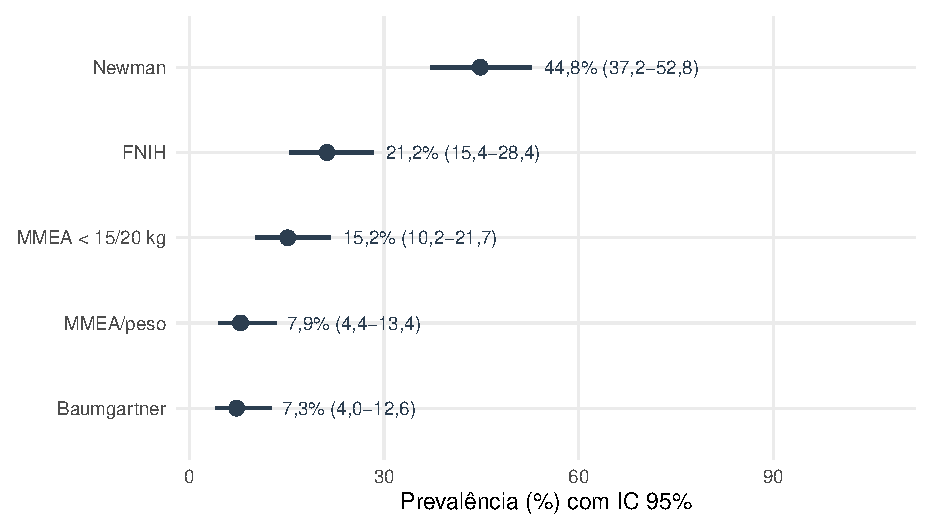
\includegraphics[width=0.85\textwidth]{outputs/figura_prevalencia_IC.pdf}
  \caption{Prevalência de baixa massa magra por critério, com IC de 95\%
           (barras de erro).}
  \label{fig:prevalencia}
\end{figure}

% ==============================================================================
\subsection{Objetivo 2: concordância entre os ajustes de MMEA}
\label{sec:obj2}
% ==============================================================================

A Tabela~\ref{tab:concordancia} resume a concordância entre os seis pares de
ajustes. Em todos os pares houve diferença estatisticamente significativa entre
as médias ($p < 0{,}001$; t pareado ou Wilcoxon). As correlações foram
moderadas a altas e todas significativas (Spearman, $r$ entre 0,36 e 0,86;
$p < 0{,}001$), indicando associação linear entre os métodos, mas associação
não implica concordância.
Optou-se pela correlação de Spearman porque as variáveis não seguem distribuição
normal (teste de Shapiro--Wilk); na matriz de correlação
(Figura~\ref{fig:correlacao}, Seção~\ref{sec:relacoes}), o coeficiente de
Pearson foi usado como medida descritiva padrão de associação linear.

A análise foi conduzida na amostra global ($n = \NTotal{}$) e validada na
subamostra com DHEM ($n = \NDHEMConcord{}$), recorte solicitado no objetivo 2;
o padrão de concordância foi idêntico (Kappa global de \KappaFleiss{} na amostra
global e \KappaFleissDHEM{} na subamostra com DHEM).

É importante notar que os ajustes comparados possuem escalas numéricas distintas
por construção: Newman expressa um resíduo de regressão linear em relação à
gordura corporal (centrado em 0), Baumgartner é um índice de massa corporal
apendicular (kg/m$^2$), FNIH é uma razão adimensional (MMEA/IMC) e MMEA/peso é
uma razão percentual. Assim, as diferenças sistemáticas de médias e as
inclinações $b \neq 1$ refletem primariamente a incompatibilidade de unidades
entre as equações, e não necessariamente discordância clínica intrínseca entre
os métodos. A métrica diagnóstica primária e clinicamente relevante é,
portanto, a concordância sobre as classificações dicotômicas, resumida pelos
coeficientes Kappa de Cohen e de Fleiss (Kappa global de \KappaFleiss{},
concordância fraca).

Na regressão sem intercepto ($Y = bX$), a hipótese $b = 1$ foi rejeitada em
cinco dos seis pares ($p < 0{,}001$). No único par em que não foi rejeitada
(Newman vs MMEA/peso, $p = 0{,}161$), a estimativa ($b = 0{,}26$) está distante
de 1 e o erro padrão é grande; não há evidência de concordância, apenas falta
de precisão. Os diagramas de Bland-Altman
(Figura~\ref{fig:bland_altman}) mostram vieses sistemáticos em todos os pares,
com limites de concordância largos, e a dispersão dos pares
(Figura~\ref{fig:conc_scatter}) evidencia retas ajustadas distantes da reta de
identidade.

Cabe um esclarecimento metodológico sobre a Figura~\ref{fig:conc_scatter} e os
pares que envolvem o método de Newman: o descolamento da reta ajustada $Y = bX$
em relação à nuvem de pontos decorre do fato de o resíduo de Newman ser centrado
em zero, enquanto as demais métricas (Baumgartner e MMEA/peso) operam em
escalas estritamente positivas. Ao forçar a reta pela origem $(0,0)$, a
regressão sem intercepto não representa adequadamente a relação contínua entre
os métodos; por isso, a avaliação de concordância diagnóstica deve se basear
nos coeficientes Kappa das classificações dicotômicas.

Os Kappas de Cohen variaram de 0,09 (Baumgartner vs MMEA/peso) a 0,48
(FNIH vs MMEA/peso), concordância fraca a moderada, e o Kappa de Fleiss
global entre os quatro critérios foi \KappaFleiss{} (concordância fraca).

\textbf{Conclusão prática:} os quatro ajustes de MMEA não são intercambiáveis.
A avaliação diagnóstica dos modelos lineares sem intercepto ($Y = bX$)
(detalhada no Apêndice~\ref{sec:apendice_concordancia}) revelou violações
severas dos pressupostos (rejeição do intercepto nulo, não normalidade e
heterocedasticidade residual). Portanto, \textbf{desaconselha-se o uso do
coeficiente $\hat{b}$ como fator de conversão matemática} entre os métodos,
devendo a avaliação de concordância restringir-se às classificações
dicotômicas (coeficientes Kappa).

\begin{table}[H]
  \centering
  \caption{Concordância entre os ajustes de MMEA (dois a dois).}
  \label{tab:concordancia}
  \resizebox{\ifdim\width>\linewidth\linewidth\else\width\fi}{!}{
\begin{tabular}[t]{lrllllll}
\toprule
Par & n & Teste de médias & Correlação & b (EP) & p (b = 1) & Kappa (Cohen) & Limites BA\\
\midrule
\cellcolor{gray!10}{Newman vs Baumgartner} & \cellcolor{gray!10}{165} & \cellcolor{gray!10}{Wilcoxon; p < 0,001} & \cellcolor{gray!10}{Spearman; r = 0,72 (p < 0,001)} & \cellcolor{gray!10}{0,080 (0,166)} & \cellcolor{gray!10}{< 0,001} & \cellcolor{gray!10}{0,15} & \cellcolor{gray!10}{2,85 a 13,55}\\
Newman vs FNIH & 165 & Wilcoxon; p < 0,001 & Spearman; r = 0,75 (p < 0,001) & 0,016 (0,014) & < 0,001 & 0,27 & -6,00 a 8,05\\
\cellcolor{gray!10}{Newman vs MMEA/peso} & \cellcolor{gray!10}{165} & \cellcolor{gray!10}{Wilcoxon; p < 0,001} & \cellcolor{gray!10}{Spearman; r = 0,82 (p < 0,001)} & \cellcolor{gray!10}{0,262 (0,523)} & \cellcolor{gray!10}{0,161} & \cellcolor{gray!10}{0,16} & \cellcolor{gray!10}{19,85 a 30,08}\\
Baumgartner vs FNIH & 165 & t pareado; p < 0,001 & Spearman; r = 0,43 (p < 0,001) & 0,080 (0,001) & < 0,001 & 0,21 & -9,91 a -4,44\\
\cellcolor{gray!10}{Baumgartner vs MMEA/peso} & \cellcolor{gray!10}{165} & \cellcolor{gray!10}{Wilcoxon; p < 0,001} & \cellcolor{gray!10}{Spearman; r = 0,36 (p < 0,001)} & \cellcolor{gray!10}{3,089 (0,046)} & \cellcolor{gray!10}{< 0,001} & \cellcolor{gray!10}{0,09} & \cellcolor{gray!10}{8,89 a 24,64}\\
FNIH vs MMEA/peso & 165 & Wilcoxon; p < 0,001 & Spearman; r = 0,86 (p < 0,001) & 37,965 (0,409) & < 0,001 & 0,48 & 15,44 a 32,43\\
\bottomrule
\end{tabular}}


  \footnotesize
  Nota: teste de médias pareado (t pareado se as diferenças são normais, senão
  Wilcoxon); correlação de Spearman (variáveis não normais) testada como $> 0$;
  regressão sem intercepto
  $Y = bX$ com teste de $b = 1$; Kappa de Cohen sobre as versões dicotômicas;
  limites de Bland-Altman (média $\pm 1{,}96$ DP das diferenças).
\end{table}

\begin{figure}[H]
  \centering
  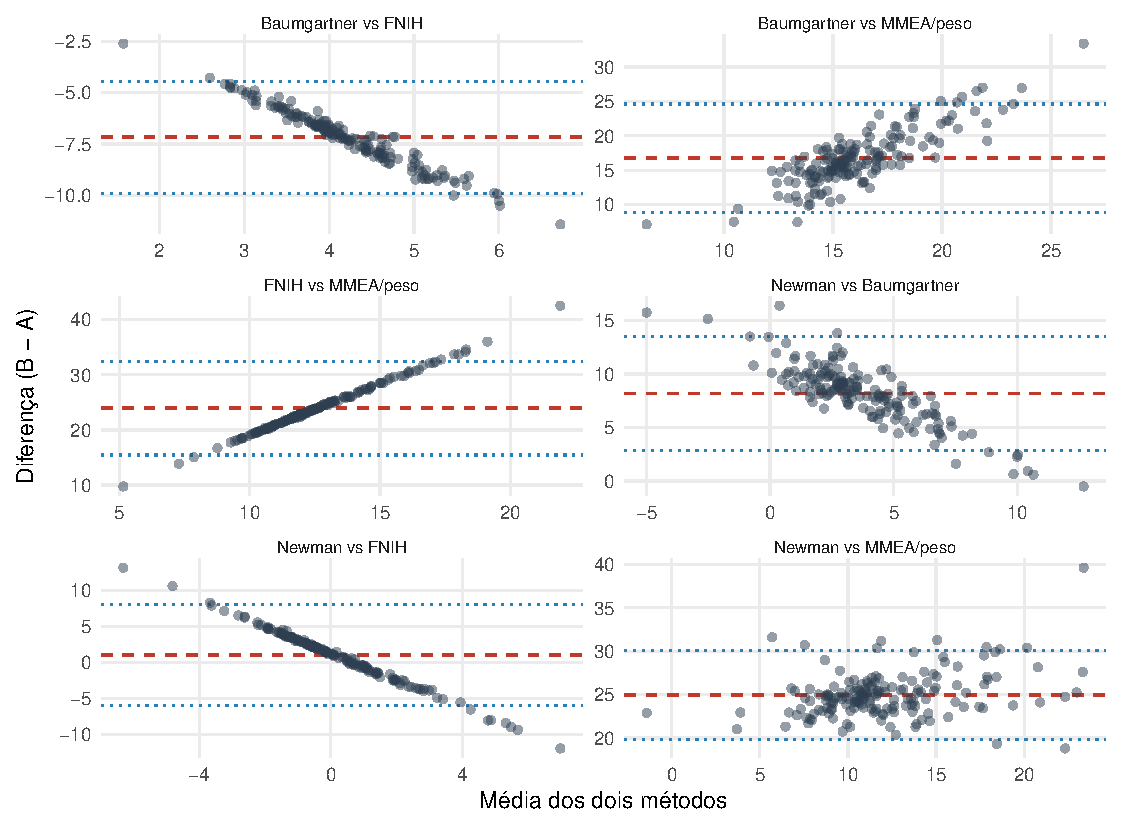
\includegraphics[width=\textwidth]{outputs/figura_bland_altman_ajustes.pdf}
  \caption{Diagramas de Bland-Altman para os seis pares de ajustes de MMEA
           (linha tracejada: viés; linhas pontilhadas: limites de concordância).}
  \label{fig:bland_altman}
\end{figure}

\begin{figure}[H]
  \centering
  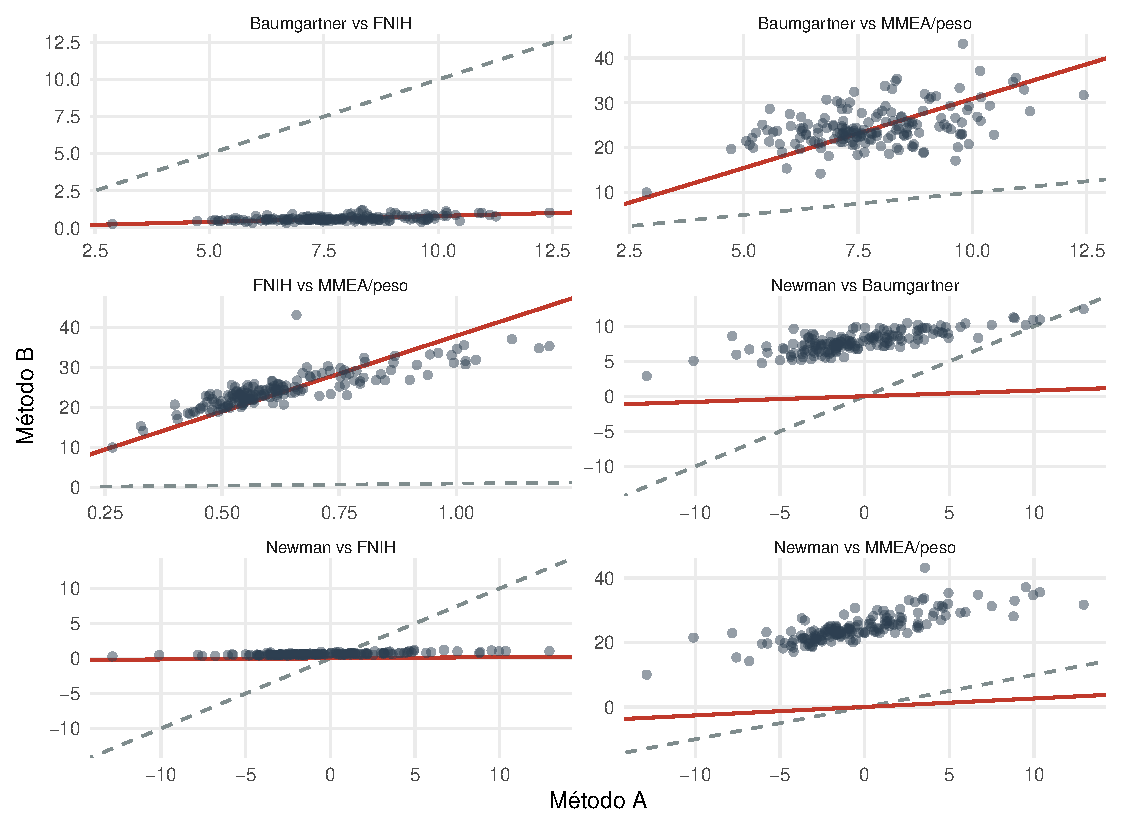
\includegraphics[width=\textwidth]{outputs/figura_concordancia_scatter.pdf}
  \caption{Dispersão dos pares de ajustes com a reta de identidade (tracejada)
           e a reta ajustada $Y = bX$ (vermelha).}
  \label{fig:conc_scatter}
\end{figure}

% ==============================================================================
\subsection{Objetivo 3: diferenças entre pacientes com e sem fibrose hepática}
\label{sec:obj3}
% ==============================================================================

A Tabela~\ref{tab:triagem_fibrose} apresenta a triagem das variáveis candidatas
para o desfecho fibrose, com $p < 0{,}20$ como critério de seleção. Foram
selecionadas oito variáveis: sexo, etnia, atividade física, obesidade, IMC,
gordura corporal (\%) e os testes funcionais de sarcopenia SARC-F $\geq 4$ e
elevação da cadeira $> 15$ s.

\begingroup\fontsize{9}{11}\selectfont

\begin{longtable}[t]{>{\raggedright\arraybackslash}p{6.2cm}>{\centering\arraybackslash}p{3.0cm}>{\centering\arraybackslash}p{3.0cm}>{\raggedleft\arraybackslash}p{2.0cm}}
\caption{Triagem de variáveis candidatas para o modelo de fibrose hepática. \label{tab:triagem_fibrose}}\\
\toprule
Característica & Não (n = 123) & Sim (n = 42) & p-valor\\
\midrule
\endfirsthead
\caption[]{Triagem de variáveis candidatas para o modelo de fibrose hepática.  \textit{(continuação)}}\\
\toprule
Característica & Não (n = 123) & Sim (n = 42) & p-valor\\
\midrule
\endhead

\endfoot
\bottomrule
\multicolumn{4}{p{0.82\linewidth}}{\rule{0pt}{1em}\raggedright{}\textit{Nota: }}\\
\multicolumn{4}{p{0.82\linewidth}}{\rule{0pt}{1em}\raggedright{}$^{1}$ Teste $t$ de Student; $^{2}$ Teste de Mann--Whitney; $^{3}$ Teste Qui-quadrado; $^{4}$ Teste Exato de Fisher. * $p < 0{,}20$: variável selecionada para a modelagem.}\\
\endlastfoot
\cellcolor{gray!10}{\textbf{Sexo$^{3}$}} & \cellcolor{gray!10}{} & \cellcolor{gray!10}{} & \cellcolor{gray!10}{\textbf{0,195*}}\\
\hspace{1em}Feminino & 95 (77,2\%) & 37 (88,1\%) & \\
\cellcolor{gray!10}{\hspace{1em}Masculino} & \cellcolor{gray!10}{28 (22,8\%)} & \cellcolor{gray!10}{5 (11,9\%)} & \cellcolor{gray!10}{}\\
\textbf{Etnia$^{4}$} &  &  & \textbf{0,018*}\\
\cellcolor{gray!10}{\hspace{1em}Branca} & \cellcolor{gray!10}{40 (32,5\%)} & \cellcolor{gray!10}{22 (52,4\%)} & \cellcolor{gray!10}{}\\
\hspace{1em}Preta & 42 (34,1\%) & 7 (16,7\%) & \\
\cellcolor{gray!10}{\hspace{1em}Parda} & \cellcolor{gray!10}{41 (33,3\%)} & \cellcolor{gray!10}{12 (28,6\%)} & \cellcolor{gray!10}{}\\
\hspace{1em}Outras & 0 (0,0\%) & 1 (2,4\%) & \\
\cellcolor{gray!10}{\textbf{Idade (anos)$^{2}$}} & \cellcolor{gray!10}{58,7 (11,2)} & \cellcolor{gray!10}{60,5 (10,6)} & \cellcolor{gray!10}{0,295}\\
\textbf{Atividade física$^{3}$} &  &  & \textbf{0,191*}\\
\cellcolor{gray!10}{\hspace{1em}Sedentário} & \cellcolor{gray!10}{78 (63,4\%)} & \cellcolor{gray!10}{33 (78,6\%)} & \cellcolor{gray!10}{}\\
\hspace{1em}\textgreater{}150 min/sem & 28 (22,8\%) & 6 (14,3\%) & \\
\cellcolor{gray!10}{\hspace{1em}\textless{}150 min/sem} & \cellcolor{gray!10}{17 (13,8\%)} & \cellcolor{gray!10}{3 (7,1\%)} & \cellcolor{gray!10}{}\\
\textbf{Tabagismo$^{4}$} &  &  & 0,358\\
\cellcolor{gray!10}{\hspace{1em}Nunca fumou} & \cellcolor{gray!10}{87 (70,7\%)} & \cellcolor{gray!10}{25 (59,5\%)} & \cellcolor{gray!10}{}\\
\hspace{1em}Fumante & 8 (6,5\%) & 3 (7,1\%) & \\
\cellcolor{gray!10}{\hspace{1em}Ex-fumante} & \cellcolor{gray!10}{28 (22,8\%)} & \cellcolor{gray!10}{14 (33,3\%)} & \cellcolor{gray!10}{}\\
\textbf{Obesidade (IMC $\geq$ 30 kg/m²)$^{3}$} &  &  & \textbf{0,051*}\\
\cellcolor{gray!10}{\hspace{1em}Não} & \cellcolor{gray!10}{52 (42,3\%)} & \cellcolor{gray!10}{10 (23,8\%)} & \cellcolor{gray!10}{}\\
\hspace{1em}Sim & 71 (57,7\%) & 32 (76,2\%) & \\
\cellcolor{gray!10}{\textbf{Sobrepeso$^{3}$}} & \cellcolor{gray!10}{} & \cellcolor{gray!10}{} & \cellcolor{gray!10}{0,274}\\
\hspace{1em}Não & 97 (78,9\%) & 37 (88,1\%) & \\
\cellcolor{gray!10}{\hspace{1em}Sim} & \cellcolor{gray!10}{26 (21,1\%)} & \cellcolor{gray!10}{5 (11,9\%)} & \cellcolor{gray!10}{}\\
\textbf{Diabetes$^{3}$} &  &  & 0,492\\
\cellcolor{gray!10}{\hspace{1em}Não} & \cellcolor{gray!10}{35 (28,5\%)} & \cellcolor{gray!10}{9 (21,4\%)} & \cellcolor{gray!10}{}\\
\hspace{1em}Sim & 88 (71,5\%) & 33 (78,6\%) & \\
\cellcolor{gray!10}{\textbf{Hipertensão arterial$^{3}$}} & \cellcolor{gray!10}{} & \cellcolor{gray!10}{} & \cellcolor{gray!10}{1,000}\\
\hspace{1em}Não & 21 (17,1\%) & 7 (16,7\%) & \\
\cellcolor{gray!10}{\hspace{1em}Sim} & \cellcolor{gray!10}{102 (82,9\%)} & \cellcolor{gray!10}{35 (83,3\%)} & \cellcolor{gray!10}{}\\
\textbf{IMC (kg/m²)$^{2}$} & 31,6 (6,1) & 34,0 (6,6) & \textbf{0,021*}\\
\cellcolor{gray!10}{\textbf{Gordura corporal (\%)$^{2}$}} & \cellcolor{gray!10}{41,8 (8,4)} & \cellcolor{gray!10}{45,2 (8,4)} & \cellcolor{gray!10}{\textbf{0,034*}}\\
\textbf{Gordura corporal$^{3}$} &  &  & 0,307\\
\cellcolor{gray!10}{\hspace{1em}Normal} & \cellcolor{gray!10}{32 (26,0\%)} & \cellcolor{gray!10}{7 (16,7\%)} & \cellcolor{gray!10}{}\\
\hspace{1em}Alta & 91 (74,0\%) & 35 (83,3\%) & \\
\cellcolor{gray!10}{\textbf{Massa magra total (kg)$^{2}$}} & \cellcolor{gray!10}{44,7 (9,4)} & \cellcolor{gray!10}{45,1 (9,0)} & \cellcolor{gray!10}{0,585}\\
\textbf{ALM/MMEA (kg)$^{2}$} & 20,0 (5,4) & 19,8 (4,8) & 0,891\\
\cellcolor{gray!10}{\textbf{Baixa massa magra (MMEA \textless{} 15/20 kg)$^{3}$}} & \cellcolor{gray!10}{} & \cellcolor{gray!10}{} & \cellcolor{gray!10}{0,667}\\
\hspace{1em}Normal & 103 (83,7\%) & 37 (88,1\%) & \\
\cellcolor{gray!10}{\hspace{1em}Reduzido} & \cellcolor{gray!10}{20 (16,3\%)} & \cellcolor{gray!10}{5 (11,9\%)} & \cellcolor{gray!10}{}\\
\textbf{MMEA reduzida (Newman)$^{3}$} &  &  & 0,338\\
\cellcolor{gray!10}{\hspace{1em}Normal} & \cellcolor{gray!10}{71 (57,7\%)} & \cellcolor{gray!10}{20 (47,6\%)} & \cellcolor{gray!10}{}\\
\hspace{1em}Reduzido & 52 (42,3\%) & 22 (52,4\%) & \\
\cellcolor{gray!10}{\textbf{Sarcopenia (Newman + handgrip)$^{3}$}} & \cellcolor{gray!10}{} & \cellcolor{gray!10}{} & \cellcolor{gray!10}{0,958}\\
\hspace{1em}Não & 106 (86,2\%) & 37 (88,1\%) & \\
\cellcolor{gray!10}{\hspace{1em}Sim} & \cellcolor{gray!10}{17 (13,8\%)} & \cellcolor{gray!10}{5 (11,9\%)} & \cellcolor{gray!10}{}\\
\textbf{MMEA reduzida (Baumgartner)$^{4}$} &  &  & 1,000\\
\cellcolor{gray!10}{\hspace{1em}Normal} & \cellcolor{gray!10}{114 (92,7\%)} & \cellcolor{gray!10}{39 (92,9\%)} & \cellcolor{gray!10}{}\\
\hspace{1em}Reduzido & 9 (7,3\%) & 3 (7,1\%) & \\
\cellcolor{gray!10}{\textbf{Sarcopenia (Baumgartner + handgrip)$^{4}$}} & \cellcolor{gray!10}{} & \cellcolor{gray!10}{} & \cellcolor{gray!10}{0,573}\\
\hspace{1em}Não & 119 (96,7\%) & 42 (100,0\%) & \\
\cellcolor{gray!10}{\hspace{1em}Sim} & \cellcolor{gray!10}{4 (3,3\%)} & \cellcolor{gray!10}{0 (0,0\%)} & \cellcolor{gray!10}{}\\
\textbf{MMEA reduzida (FNIH)$^{3}$} &  &  & 0,257\\
\cellcolor{gray!10}{\hspace{1em}Normal} & \cellcolor{gray!10}{100 (81,3\%)} & \cellcolor{gray!10}{30 (71,4\%)} & \cellcolor{gray!10}{}\\
\hspace{1em}Reduzido & 23 (18,7\%) & 12 (28,6\%) & \\
\cellcolor{gray!10}{\textbf{Sarcopenia (FNIH + handgrip)$^{4}$}} & \cellcolor{gray!10}{} & \cellcolor{gray!10}{} & \cellcolor{gray!10}{0,741}\\
\hspace{1em}Não & 114 (92,7\%) & 38 (90,5\%) & \\
\cellcolor{gray!10}{\hspace{1em}Sim} & \cellcolor{gray!10}{9 (7,3\%)} & \cellcolor{gray!10}{4 (9,5\%)} & \cellcolor{gray!10}{}\\
\textbf{MMEA reduzida (peso)$^{4}$} &  &  & 0,319\\
\cellcolor{gray!10}{\hspace{1em}Normal} & \cellcolor{gray!10}{115 (93,5\%)} & \cellcolor{gray!10}{37 (88,1\%)} & \cellcolor{gray!10}{}\\
\hspace{1em}Reduzido & 8 (6,5\%) & 5 (11,9\%) & \\
\cellcolor{gray!10}{\textbf{Sarcopenia (SARC-F $\geq$ 4)$^{3}$}} & \cellcolor{gray!10}{} & \cellcolor{gray!10}{} & \cellcolor{gray!10}{\textbf{0,176*}}\\
\hspace{1em}Normal & 83 (76,1\%) & 26 (63,4\%) & \\
\cellcolor{gray!10}{\hspace{1em}Alterado} & \cellcolor{gray!10}{26 (23,9\%)} & \cellcolor{gray!10}{15 (36,6\%)} & \cellcolor{gray!10}{}\\
\textbf{Sarcopenia (SARC-F + panturrilha $\geq$ 11)$^{3}$} &  &  & 1,000\\
\cellcolor{gray!10}{\hspace{1em}Normal} & \cellcolor{gray!10}{86 (80,4\%)} & \cellcolor{gray!10}{33 (80,5\%)} & \cellcolor{gray!10}{}\\
\hspace{1em}Alterado & 21 (19,6\%) & 8 (19,5\%) & \\
\cellcolor{gray!10}{\textbf{Sarcopenia (handgrip \textless{} 16/27 kg)$^{3}$}} & \cellcolor{gray!10}{} & \cellcolor{gray!10}{} & \cellcolor{gray!10}{0,514}\\
\hspace{1em}Normal & 66 (68,0\%) & 28 (75,7\%) & \\
\cellcolor{gray!10}{\hspace{1em}Alterado} & \cellcolor{gray!10}{31 (32,0\%)} & \cellcolor{gray!10}{9 (24,3\%)} & \cellcolor{gray!10}{}\\
\textbf{Sarcopenia (elevação da cadeira \textgreater{} 15 s)$^{3}$} &  &  & \textbf{0,060*}\\
\cellcolor{gray!10}{\hspace{1em}Normal} & \cellcolor{gray!10}{57 (57,6\%)} & \cellcolor{gray!10}{13 (37,1\%)} & \cellcolor{gray!10}{}\\
\hspace{1em}Alterado & 42 (42,4\%) & 22 (62,9\%) & \\
\cellcolor{gray!10}{\textbf{Sarcopenia (velocidade de marcha \textless{} 0,8 m/s)$^{3}$}} & \cellcolor{gray!10}{} & \cellcolor{gray!10}{} & \cellcolor{gray!10}{0,847}\\
\hspace{1em}Normal & 22 (23,2\%) & 6 (19,4\%) & \\
\cellcolor{gray!10}{\hspace{1em}Alterado} & \cellcolor{gray!10}{73 (76,8\%)} & \cellcolor{gray!10}{25 (80,6\%)} & \cellcolor{gray!10}{}\\*
\end{longtable}
\endgroup{}


Para cada uma dessas covariáveis selecionadas, ajustou-se previamente um modelo
logístico simples; as razões de chances (OR) não ajustadas e seus IC 95\% são
resumidos na Tabela~\ref{tab:modelo_simples_fibrose}. Os termos em negrito
indicam as variáveis retidas no modelo múltiplo pela seleção stepwise.

\begin{table}[H]
  \centering
  \caption{Modelos logísticos simples para fibrose hepática.}
  \label{tab:modelo_simples_fibrose}
  \begingroup\setlength{\tabcolsep}{1.5pt}\begin{tabular}[t]{>{\raggedright\arraybackslash}p{6.5cm}>{\centering\arraybackslash}p{3.0cm}>{\centering\arraybackslash}p{3.0cm}>{\centering\arraybackslash}p{3.0cm}}
\toprule
Variável & OR & IC 95\% & p-valor\\
\midrule
\cellcolor{gray!10}{Sexo (Masculino vs. Feminino)} & \cellcolor{gray!10}{0,75} & \cellcolor{gray!10}{0,23–2,07} & \cellcolor{gray!10}{0,600}\\
\textbf{Etnia (Ref.: Branca)} &  &  & \\
\cellcolor{gray!10}{\hspace{1em}Preta} & \cellcolor{gray!10}{0,25} & \cellcolor{gray!10}{0,08–0,67} & \cellcolor{gray!10}{\textbf{0,009}}\\
\hspace{1em}Parda & 0,43 & 0,16–1,10 & \textbf{0,086}\\
\cellcolor{gray!10}{\textbf{Atividade física (Ref.: Sedentário)}} & \cellcolor{gray!10}{} & \cellcolor{gray!10}{} & \cellcolor{gray!10}{}\\
\hspace{1em}\textgreater{}150 min/sem & 0,60 & 0,20–1,58 & 0,324\\
\cellcolor{gray!10}{\hspace{1em}\textless{}150 min/sem} & \cellcolor{gray!10}{0,43} & \cellcolor{gray!10}{0,09–1,44} & \cellcolor{gray!10}{0,212}\\
Obesidade (IMC $\geq$ 30 kg/m²) (Sim vs. Não) & 2,59 & 1,11–6,62 & 0,035\\
\cellcolor{gray!10}{IMC (kg/m²)} & \cellcolor{gray!10}{1,06} & \cellcolor{gray!10}{0,99–1,12} & \cellcolor{gray!10}{\textbf{0,078}}\\
Gordura corporal (\%) & 1,04 & 0,99–1,09 & 0,136\\
\cellcolor{gray!10}{Sarcopenia (SARC-F $\geq$ 4) (Alterado vs. Normal)} & \cellcolor{gray!10}{1,72} & \cellcolor{gray!10}{0,73–3,97} & \cellcolor{gray!10}{0,204}\\
Sarcopenia (elevação da cadeira \textgreater{} 15 s) (Alterado vs. Normal) & 2,30 & 1,05–5,18 & \textbf{0,040}\\
\bottomrule
\multicolumn{4}{p{0.82\linewidth}}{\rule{0pt}{1em}\raggedright{}\textit{Nota: }}\\
\multicolumn{4}{p{0.82\linewidth}}{\rule{0pt}{1em}\raggedright{}Modelos logísticos simples para cada covariável selecionada na triagem (p < 0,20). Em negrito, as covariáveis retidas no modelo múltiplo por stepwise (critério AIC).}\\
\end{tabular}\endgroup

\end{table}

Em seguida, ajustou-se o modelo logístico múltiplo com todas as variáveis
triadas, submetido à seleção stepwise (direção \textit{both}, critério AIC);
o modelo final para fibrose
(Tabela~\ref{tab:modelo_fibrose}; $n = 134$) reteve etnia, IMC e a alteração no
teste de elevação da cadeira.
Pacientes de etnia preta apresentaram menor chance de fibrose em relação aos
brancos (OR = 0,24; IC 95\%: 0,08--0,66; $p = 0{,}008$); para pardos, a diferença
não foi significativa (OR = 0,42; IC 95\%: 0,15--1,10; $p = 0{,}086$); cada
aumento de 1 kg/m$^2$ no IMC associou-se a um aumento estimado de 5\% na chance
de fibrose, sem significância estatística (OR = 1,05; IC 95\%: 0,99--1,13;
$p = 0{,}109$); e a alteração no teste de elevação da cadeira mais que dobrou a
chance de fibrose, também sem significância estatística (OR = 2,11;
IC 95\%: 0,93--4,95; $p = 0{,}078$).

Em relação à pergunta central do objetivo, a hipótese nula de ausência de
diferença não foi rejeitada para a quantidade de massa muscular: a massa magra
total foi de 45,1 kg (DP = 9,0) nos pacientes com fibrose e 44,7 kg (DP = 9,4)
nos sem fibrose ($p = 0{,}585$), e o ALM/MMEA foi de 19,8 kg (DP = 4,8) contra
20,0 kg (DP = 5,4) ($p = 0{,}891$). Após controlar pelos confundidores clássicos
(sexo, idade e IMC) em um modelo de regressão logística múltiplo, a fibrose
permaneceu sem associação estatisticamente significativa com a massa magra
total ($\beta \approx \BetaFibroseMMT{}$ kg; $p = \PBetaFibroseMMT{}$).

O impacto muscular associado à fibrose manifestou-se, porém, no desempenho
funcional: a alteração no teste de elevação da cadeira foi de 62,9\% no grupo
com fibrose contra 42,4\% no grupo sem fibrose ($p = 0{,}060$). Em conjunto,
esses resultados indicam que a fibrose hepática está associada a perdas de
desempenho e força física funcional, e não necessariamente à redução do volume
bruto de massa magra.

\begin{table}[H]
  \centering
  \caption{Modelo de regressão logística múltipla para fibrose hepática.}
  \label{tab:modelo_fibrose}
  \begingroup\setlength{\tabcolsep}{1.5pt}\begin{tabular}[t]{>{\raggedright\arraybackslash}p{6.5cm}>{\centering\arraybackslash}p{3.0cm}>{\centering\arraybackslash}p{3.0cm}>{\centering\arraybackslash}p{3.0cm}}
\toprule
Variável & OR & IC 95\% & p-valor\\
\midrule
\cellcolor{gray!10}{\textbf{Etnia (Ref.: Branca)}} & \cellcolor{gray!10}{} & \cellcolor{gray!10}{} & \cellcolor{gray!10}{}\\
\hspace{1em}Preta & 0,24 & 0,08–0,66 & 0,008\\
\cellcolor{gray!10}{\hspace{1em}Parda} & \cellcolor{gray!10}{0,42} & \cellcolor{gray!10}{0,15–1,10} & \cellcolor{gray!10}{0,086}\\
IMC (kg/m²) & 1,05 & 0,99–1,13 & 0,109\\
\cellcolor{gray!10}{Sarcopenia (elevação da cadeira \textgreater{} 15 s) (Alterado vs. Normal)} & \cellcolor{gray!10}{2,11} & \cellcolor{gray!10}{0,93–4,95} & \cellcolor{gray!10}{0,078}\\
\bottomrule
\end{tabular}\endgroup


  \footnotesize
  Nota: 1 paciente da categoria ``Outras'' (etnia, $n = 1$) foi excluído por
  ser categoria esparsa. Referência da etnia: branca.
\end{table}

% ==============================================================================
\subsection{Objetivo 4: diferenças entre pacientes com e sem DHEM}
\label{sec:obj4}
% ==============================================================================

A triagem (Tabela~\ref{tab:triagem_dhem}) selecionou onze variáveis com
$p < 0{,}20$: etnia, idade, atividade física, obesidade, IMC, gordura corporal
(\%), gordura corporal (categorizada), massa magra total (kg), MMEA reduzida
(peso) e os testes funcionais de elevação da cadeira e velocidade de marcha.

\begingroup\fontsize{9}{11}\selectfont

\begin{longtable}[t]{>{\raggedright\arraybackslash}p{6.2cm}>{\centering\arraybackslash}p{3.0cm}>{\centering\arraybackslash}p{3.0cm}>{\raggedleft\arraybackslash}p{2.0cm}}
\caption{Triagem de variáveis candidatas para o modelo de DHEM. \label{tab:triagem_dhem}}\\
\toprule
Característica & Não (n = 27) & Sim (n = 138) & p-valor\\
\midrule
\endfirsthead
\caption[]{Triagem de variáveis candidatas para o modelo de DHEM.  \textit{(continuação)}}\\
\toprule
Característica & Não (n = 27) & Sim (n = 138) & p-valor\\
\midrule
\endhead

\endfoot
\bottomrule
\multicolumn{4}{p{0.82\linewidth}}{\rule{0pt}{1em}\raggedright{}\textit{Nota: }}\\
\multicolumn{4}{p{0.82\linewidth}}{\rule{0pt}{1em}\raggedright{}$^{1}$ Teste $t$ de Student; $^{2}$ Teste de Mann--Whitney; $^{3}$ Teste Qui-quadrado; $^{4}$ Teste Exato de Fisher. * $p < 0{,}20$: variável selecionada para a modelagem.}\\
\endlastfoot
\cellcolor{gray!10}{\textbf{Sexo$^{3}$}} & \cellcolor{gray!10}{} & \cellcolor{gray!10}{} & \cellcolor{gray!10}{0,958}\\
\hspace{1em}Feminino & 21 (77,8\%) & 111 (80,4\%) & \\
\cellcolor{gray!10}{\hspace{1em}Masculino} & \cellcolor{gray!10}{6 (22,2\%)} & \cellcolor{gray!10}{27 (19,6\%)} & \cellcolor{gray!10}{}\\
\textbf{Etnia$^{4}$} &  &  & \textbf{0,048*}\\
\cellcolor{gray!10}{\hspace{1em}Branca} & \cellcolor{gray!10}{7 (25,9\%)} & \cellcolor{gray!10}{55 (39,9\%)} & \cellcolor{gray!10}{}\\
\hspace{1em}Preta & 12 (44,4\%) & 37 (26,8\%) & \\
\cellcolor{gray!10}{\hspace{1em}Parda} & \cellcolor{gray!10}{7 (25,9\%)} & \cellcolor{gray!10}{46 (33,3\%)} & \cellcolor{gray!10}{}\\
\hspace{1em}Outras & 1 (3,7\%) & 0 (0,0\%) & \\
\cellcolor{gray!10}{\textbf{Idade (anos)$^{2}$}} & \cellcolor{gray!10}{62,7 (9,0)} & \cellcolor{gray!10}{58,5 (11,3)} & \cellcolor{gray!10}{\textbf{0,089*}}\\
\textbf{Atividade física$^{4}$} &  &  & \textbf{0,041*}\\
\cellcolor{gray!10}{\hspace{1em}Sedentário} & \cellcolor{gray!10}{13 (48,1\%)} & \cellcolor{gray!10}{98 (71,0\%)} & \cellcolor{gray!10}{}\\
\hspace{1em}\textgreater{}150 min/sem & 10 (37,0\%) & 24 (17,4\%) & \\
\cellcolor{gray!10}{\hspace{1em}\textless{}150 min/sem} & \cellcolor{gray!10}{4 (14,8\%)} & \cellcolor{gray!10}{16 (11,6\%)} & \cellcolor{gray!10}{}\\
\textbf{Tabagismo$^{4}$} &  &  & 0,596\\
\cellcolor{gray!10}{\hspace{1em}Nunca fumou} & \cellcolor{gray!10}{17 (63,0\%)} & \cellcolor{gray!10}{95 (68,8\%)} & \cellcolor{gray!10}{}\\
\hspace{1em}Fumante & 1 (3,7\%) & 10 (7,2\%) & \\
\cellcolor{gray!10}{\hspace{1em}Ex-fumante} & \cellcolor{gray!10}{9 (33,3\%)} & \cellcolor{gray!10}{33 (23,9\%)} & \cellcolor{gray!10}{}\\
\textbf{Obesidade (IMC $\geq$ 30 kg/m²)$^{3}$} &  &  & \textbf{0,006*}\\
\cellcolor{gray!10}{\hspace{1em}Não} & \cellcolor{gray!10}{17 (63,0\%)} & \cellcolor{gray!10}{45 (32,6\%)} & \cellcolor{gray!10}{}\\
\hspace{1em}Sim & 10 (37,0\%) & 93 (67,4\%) & \\
\cellcolor{gray!10}{\textbf{Sobrepeso$^{3}$}} & \cellcolor{gray!10}{} & \cellcolor{gray!10}{} & \cellcolor{gray!10}{0,397}\\
\hspace{1em}Não & 24 (88,9\%) & 110 (79,7\%) & \\
\cellcolor{gray!10}{\hspace{1em}Sim} & \cellcolor{gray!10}{3 (11,1\%)} & \cellcolor{gray!10}{28 (20,3\%)} & \cellcolor{gray!10}{}\\
\textbf{Diabetes$^{3}$} &  &  & 0,536\\
\cellcolor{gray!10}{\hspace{1em}Não} & \cellcolor{gray!10}{9 (33,3\%)} & \cellcolor{gray!10}{35 (25,4\%)} & \cellcolor{gray!10}{}\\
\hspace{1em}Sim & 18 (66,7\%) & 103 (74,6\%) & \\
\cellcolor{gray!10}{\textbf{Hipertensão arterial$^{4}$}} & \cellcolor{gray!10}{} & \cellcolor{gray!10}{} & \cellcolor{gray!10}{0,575}\\
\hspace{1em}Não & 3 (11,1\%) & 25 (18,1\%) & \\
\cellcolor{gray!10}{\hspace{1em}Sim} & \cellcolor{gray!10}{24 (88,9\%)} & \cellcolor{gray!10}{113 (81,9\%)} & \cellcolor{gray!10}{}\\
\textbf{IMC (kg/m²)$^{2}$} & 28,8 (5,7) & 32,9 (6,2) & \textbf{\textless{} 0,001*}\\
\cellcolor{gray!10}{\textbf{Gordura corporal (\%)$^{2}$}} & \cellcolor{gray!10}{38,4 (11,2)} & \cellcolor{gray!10}{43,5 (7,6)} & \cellcolor{gray!10}{\textbf{0,042*}}\\
\textbf{Gordura corporal$^{3}$} &  &  & \textbf{0,011*}\\
\cellcolor{gray!10}{\hspace{1em}Normal} & \cellcolor{gray!10}{12 (44,4\%)} & \cellcolor{gray!10}{27 (19,6\%)} & \cellcolor{gray!10}{}\\
\hspace{1em}Alta & 15 (55,6\%) & 111 (80,4\%) & \\
\cellcolor{gray!10}{\textbf{Massa magra total (kg)$^{2}$}} & \cellcolor{gray!10}{42,3 (9,4)} & \cellcolor{gray!10}{45,3 (9,3)} & \cellcolor{gray!10}{\textbf{0,103*}}\\
\textbf{ALM/MMEA (kg)$^{2}$} & 19,1 (5,2) & 20,2 (5,2) & 0,352\\
\cellcolor{gray!10}{\textbf{Baixa massa magra (MMEA \textless{} 15/20 kg)$^{4}$}} & \cellcolor{gray!10}{} & \cellcolor{gray!10}{} & \cellcolor{gray!10}{0,565}\\
\hspace{1em}Normal & 22 (81,5\%) & 118 (85,5\%) & \\
\cellcolor{gray!10}{\hspace{1em}Reduzido} & \cellcolor{gray!10}{5 (18,5\%)} & \cellcolor{gray!10}{20 (14,5\%)} & \cellcolor{gray!10}{}\\
\textbf{MMEA reduzida (Newman)$^{3}$} &  &  & 0,869\\
\cellcolor{gray!10}{\hspace{1em}Normal} & \cellcolor{gray!10}{14 (51,9\%)} & \cellcolor{gray!10}{77 (55,8\%)} & \cellcolor{gray!10}{}\\
\hspace{1em}Reduzido & 13 (48,1\%) & 61 (44,2\%) & \\
\cellcolor{gray!10}{\textbf{Sarcopenia (Newman + handgrip)$^{4}$}} & \cellcolor{gray!10}{} & \cellcolor{gray!10}{} & \cellcolor{gray!10}{0,762}\\
\hspace{1em}Não & 23 (85,2\%) & 120 (87,0\%) & \\
\cellcolor{gray!10}{\hspace{1em}Sim} & \cellcolor{gray!10}{4 (14,8\%)} & \cellcolor{gray!10}{18 (13,0\%)} & \cellcolor{gray!10}{}\\
\textbf{MMEA reduzida (Baumgartner)$^{4}$} &  &  & 0,417\\
\cellcolor{gray!10}{\hspace{1em}Normal} & \cellcolor{gray!10}{24 (88,9\%)} & \cellcolor{gray!10}{129 (93,5\%)} & \cellcolor{gray!10}{}\\
\hspace{1em}Reduzido & 3 (11,1\%) & 9 (6,5\%) & \\
\cellcolor{gray!10}{\textbf{Sarcopenia (Baumgartner + handgrip)$^{4}$}} & \cellcolor{gray!10}{} & \cellcolor{gray!10}{} & \cellcolor{gray!10}{1,000}\\
\hspace{1em}Não & 27 (100,0\%) & 134 (97,1\%) & \\
\cellcolor{gray!10}{\hspace{1em}Sim} & \cellcolor{gray!10}{0 (0,0\%)} & \cellcolor{gray!10}{4 (2,9\%)} & \cellcolor{gray!10}{}\\
\textbf{MMEA reduzida (FNIH)$^{3}$} &  &  & 0,528\\
\cellcolor{gray!10}{\hspace{1em}Normal} & \cellcolor{gray!10}{23 (85,2\%)} & \cellcolor{gray!10}{107 (77,5\%)} & \cellcolor{gray!10}{}\\
\hspace{1em}Reduzido & 4 (14,8\%) & 31 (22,5\%) & \\
\cellcolor{gray!10}{\textbf{Sarcopenia (FNIH + handgrip)$^{4}$}} & \cellcolor{gray!10}{} & \cellcolor{gray!10}{} & \cellcolor{gray!10}{0,696}\\
\hspace{1em}Não & 26 (96,3\%) & 126 (91,3\%) & \\
\cellcolor{gray!10}{\hspace{1em}Sim} & \cellcolor{gray!10}{1 (3,7\%)} & \cellcolor{gray!10}{12 (8,7\%)} & \cellcolor{gray!10}{}\\
\textbf{MMEA reduzida (peso)$^{4}$} &  &  & \textbf{0,130*}\\
\cellcolor{gray!10}{\hspace{1em}Normal} & \cellcolor{gray!10}{27 (100,0\%)} & \cellcolor{gray!10}{125 (90,6\%)} & \cellcolor{gray!10}{}\\
\hspace{1em}Reduzido & 0 (0,0\%) & 13 (9,4\%) & \\
\cellcolor{gray!10}{\textbf{Sarcopenia (SARC-F $\geq$ 4)$^{3}$}} & \cellcolor{gray!10}{} & \cellcolor{gray!10}{} & \cellcolor{gray!10}{0,303}\\
\hspace{1em}Normal & 20 (83,3\%) & 89 (70,6\%) & \\
\cellcolor{gray!10}{\hspace{1em}Alterado} & \cellcolor{gray!10}{4 (16,7\%)} & \cellcolor{gray!10}{37 (29,4\%)} & \cellcolor{gray!10}{}\\
\textbf{Sarcopenia (SARC-F + panturrilha $\geq$ 11)$^{4}$} &  &  & 0,259\\
\cellcolor{gray!10}{\hspace{1em}Normal} & \cellcolor{gray!10}{17 (70,8\%)} & \cellcolor{gray!10}{102 (82,3\%)} & \cellcolor{gray!10}{}\\
\hspace{1em}Alterado & 7 (29,2\%) & 22 (17,7\%) & \\
\cellcolor{gray!10}{\textbf{Sarcopenia (handgrip \textless{} 16/27 kg)$^{3}$}} & \cellcolor{gray!10}{} & \cellcolor{gray!10}{} & \cellcolor{gray!10}{1,000}\\
\hspace{1em}Normal & 15 (68,2\%) & 79 (70,5\%) & \\
\cellcolor{gray!10}{\hspace{1em}Alterado} & \cellcolor{gray!10}{7 (31,8\%)} & \cellcolor{gray!10}{33 (29,5\%)} & \cellcolor{gray!10}{}\\
\textbf{Sarcopenia (elevação da cadeira \textgreater{} 15 s)$^{3}$} &  &  & \textbf{0,160*}\\
\cellcolor{gray!10}{\hspace{1em}Normal} & \cellcolor{gray!10}{15 (68,2\%)} & \cellcolor{gray!10}{55 (49,1\%)} & \cellcolor{gray!10}{}\\
\hspace{1em}Alterado & 7 (31,8\%) & 57 (50,9\%) & \\
\cellcolor{gray!10}{\textbf{Sarcopenia (velocidade de marcha \textless{} 0,8 m/s)$^{4}$}} & \cellcolor{gray!10}{} & \cellcolor{gray!10}{} & \cellcolor{gray!10}{\textbf{0,020*}}\\
\hspace{1em}Normal & 9 (42,9\%) & 19 (18,1\%) & \\
\cellcolor{gray!10}{\hspace{1em}Alterado} & \cellcolor{gray!10}{12 (57,1\%)} & \cellcolor{gray!10}{86 (81,9\%)} & \cellcolor{gray!10}{}\\*
\end{longtable}
\endgroup{}


A Tabela~\ref{tab:modelo_simples_dhem} resume os modelos logísticos simples para
cada uma dessas covariáveis selecionadas. Nela, observa-se que a MMEA reduzida
(peso) apresentou estimativas numericamente instáveis (OR extremamente elevado e
IC 95\% não finito), decorrentes da quase-separação provocada por caselas
esparsas; por isso, essa variável não foi retida na seleção stepwise e não
compôs o modelo múltiplo final, e seus resultados não devem ser interpretados
clinicamente (ver Seção~\ref{sec:discussao}).

\begin{table}[H]
  \centering
  \caption{Modelos logísticos simples para DHEM.}
  \label{tab:modelo_simples_dhem}
  \begingroup\setlength{\tabcolsep}{1.5pt}\begin{tabular}[t]{>{\raggedright\arraybackslash}p{6.5cm}>{\centering\arraybackslash}p{3.0cm}>{\centering\arraybackslash}p{3.0cm}>{\centering\arraybackslash}p{3.0cm}}
\toprule
Variável & OR & IC 95\% & p-valor\\
\midrule
\cellcolor{gray!10}{\textbf{Etnia (Ref.: Branca)}} & \cellcolor{gray!10}{} & \cellcolor{gray!10}{} & \cellcolor{gray!10}{}\\
\hspace{1em}Preta & 0,37 & 0,12–1,08 & 0,075\\
\cellcolor{gray!10}{\hspace{1em}Parda} & \cellcolor{gray!10}{1,08} & \cellcolor{gray!10}{0,28–4,53} & \cellcolor{gray!10}{0,909}\\
Idade (anos) & 0,97 & 0,92–1,01 & \textbf{0,153}\\
\cellcolor{gray!10}{\textbf{Atividade física (Ref.: Sedentário)}} & \cellcolor{gray!10}{} & \cellcolor{gray!10}{} & \cellcolor{gray!10}{}\\
\hspace{1em}\textgreater{}150 min/sem & 0,29 & 0,10–0,82 & \textbf{0,019}\\
\cellcolor{gray!10}{\hspace{1em}\textless{}150 min/sem} & \cellcolor{gray!10}{0,56} & \cellcolor{gray!10}{0,14–2,76} & \cellcolor{gray!10}{\textbf{0,424}}\\
Obesidade (IMC $\geq$ 30 kg/m²) (Sim vs. Não) & 3,30 & 1,27–9,06 & 0,016\\
\cellcolor{gray!10}{IMC (kg/m²)} & \cellcolor{gray!10}{1,12} & \cellcolor{gray!10}{1,03–1,25} & \cellcolor{gray!10}{0,019}\\
Gordura corporal (\%) & 1,07 & 1,02–1,13 & \textbf{0,012}\\
\cellcolor{gray!10}{Gordura corporal (Alta vs. Normal)} & \cellcolor{gray!10}{2,61} & \cellcolor{gray!10}{0,96–6,96} & \cellcolor{gray!10}{0,055}\\
Massa magra total (kg) & 1,03 & 0,97–1,10 & 0,371\\
\cellcolor{gray!10}{MMEA reduzida (peso) (Reduzido vs. Normal)} & \cellcolor{gray!10}{9504692,11} & \cellcolor{gray!10}{0,00–—} & \cellcolor{gray!10}{0,990}\\
Sarcopenia (elevação da cadeira \textgreater{} 15 s) (Alterado vs. Normal) & 2,36 & 0,88–7,05 & 0,100\\
\cellcolor{gray!10}{Sarcopenia (velocidade de marcha \textless{} 0,8 m/s) (Alterado vs. Normal)} & \cellcolor{gray!10}{3,32} & \cellcolor{gray!10}{1,20–9,01} & \cellcolor{gray!10}{\textbf{0,018}}\\
\bottomrule
\multicolumn{4}{p{0.82\linewidth}}{\rule{0pt}{1em}\raggedright{}\textit{Nota: }}\\
\multicolumn{4}{p{0.82\linewidth}}{\rule{0pt}{1em}\raggedright{}Modelos logísticos simples para cada covariável selecionada na triagem (p < 0,20). Em negrito, as covariáveis retidas no modelo múltiplo por stepwise (critério AIC).}\\
\end{tabular}\endgroup

\end{table}

O modelo final por stepwise (Tabela~\ref{tab:modelo_dhem}; $n = 124$) reteve
idade, atividade física, gordura corporal (\%) e velocidade de marcha alterada.
Cada ano adicional de idade associou-se a menor chance de DHEM (OR = 0,94;
IC 95\%: 0,89--0,99; $p = 0{,}032$); a atividade física intensa
($> 150$ min/sem) reduziu a chance de DHEM em relação ao sedentarismo
(OR = 0,22; IC 95\%: 0,06--0,75; $p = 0{,}017$); cada ponto percentual adicional
de gordura corporal aumentou a chance de DHEM em 7\% (OR = 1,07;
IC 95\%: 1,01--1,14; $p = 0{,}029$); e a velocidade de marcha alterada quase
triplicou a chance de DHEM (OR = 2,83; IC 95\%: 0,90--8,79; $p = 0{,}070$).

\begin{table}[H]
  \centering
  \caption{Modelo de regressão logística múltipla para DHEM.}
  \label{tab:modelo_dhem}
  \begingroup\setlength{\tabcolsep}{1.5pt}\begin{tabular}[t]{>{\raggedright\arraybackslash}p{6.5cm}>{\centering\arraybackslash}p{3.0cm}>{\centering\arraybackslash}p{3.0cm}>{\centering\arraybackslash}p{3.0cm}}
\toprule
Variável & OR & IC 95\% & p-valor\\
\midrule
\cellcolor{gray!10}{Idade (anos)} & \cellcolor{gray!10}{0,94} & \cellcolor{gray!10}{0,89–0,99} & \cellcolor{gray!10}{0,032}\\
\textbf{Atividade física (Ref.: Sedentário)} &  &  & \\
\cellcolor{gray!10}{\hspace{1em}\textgreater{}150 min/sem} & \cellcolor{gray!10}{0,22} & \cellcolor{gray!10}{0,06–0,75} & \cellcolor{gray!10}{0,017}\\
\hspace{1em}\textless{}150 min/sem & 0,52 & 0,12–2,86 & 0,412\\
\cellcolor{gray!10}{Gordura corporal (\%)} & \cellcolor{gray!10}{1,07} & \cellcolor{gray!10}{1,01–1,14} & \cellcolor{gray!10}{0,029}\\
Sarcopenia (velocidade de marcha \textless{} 0,8 m/s) (Alterado vs. Normal) & 2,83 & 0,90–8,79 & 0,070\\
\bottomrule
\end{tabular}\endgroup

\end{table}

% ==============================================================================
\subsection{Objetivo 5: comparação dos três grupos (DHEM/fibrose)}
\label{sec:obj5}
% ==============================================================================

A Tabela~\ref{tab:testes_grupos} resume os testes de hipóteses para comparação
dos três grupos. Entre as variáveis numéricas, o IMC (Kruskal--Wallis:
$H = 9{,}72$; $p = 0{,}008$) e a gordura corporal ($p = 0{,}045$) diferiram
entre os grupos; idade, massa magra total e ALM/MMEA foram semelhantes. Entre
as categóricas, a obesidade diferiu
($\chi^2 = 7{,}78$; $p = 0{,}020$), consistente com o gradiente observado na
Tabela~\ref{tab:cruzamento}; diabetes, hipertensão e os critérios de sarcopenia
não diferiram significativamente entre os grupos.

\begingroup\fontsize{9}{11}\selectfont

\begin{longtable}[t]{>{\raggedright\arraybackslash}p{6.5cm}>{\raggedright\arraybackslash}p{3.0cm}>{\raggedright\arraybackslash}p{2.5cm}>{\raggedright\arraybackslash}p{2.0cm}}
\caption{Testes de hipóteses para comparação dos três grupos de DHEM/fibrose (objetivo 5). Numéricas: ANOVA (normalidade) ou Kruskal-Wallis; categóricas: qui-quadrado ou Fisher (contagens esperadas \textless{} 5). \label{tab:testes_grupos}}\\
\toprule
Variável & Teste & Estatística & valor-p\\
\midrule
\endfirsthead
\caption[]{Testes de hipóteses para comparação dos três grupos de DHEM/fibrose (objetivo 5). Numéricas: ANOVA (normalidade) ou Kruskal-Wallis; categóricas: qui-quadrado ou Fisher (contagens esperadas \textless{} 5).  \textit{(continuação)}}\\
\toprule
Variável & Teste & Estatística & valor-p\\
\midrule
\endhead

\endfoot
\bottomrule
\multicolumn{4}{p{0.82\linewidth}}{\rule{0pt}{1em}\raggedright{}\textit{Nota: }}\\
\multicolumn{4}{p{0.82\linewidth}}{\rule{0pt}{1em}\raggedright{}$^{1}$ Teste $t$ de Student; $^{2}$ Teste de Mann--Whitney; $^{3}$ Teste Qui-quadrado; $^{4}$ Teste Exato de Fisher; $^{5}$ ANOVA; $^{6}$ Kruskal--Wallis.}\\
\endlastfoot
\addlinespace[0.3em]
\multicolumn{4}{l}{\textbf{Características sociodemográficas}}\\
\hspace{1em}\cellcolor{gray!10}{Sexo$^{4}$} & \cellcolor{gray!10}{Fisher (exato)} & \cellcolor{gray!10}{—} & \cellcolor{gray!10}{0,315}\\
\hspace{1em}Etnia$^{4}$ & Fisher (exato) & — & 0,057\\
\hspace{1em}\cellcolor{gray!10}{Idade (anos)$^{6}$} & \cellcolor{gray!10}{Kruskal-Wallis} & \cellcolor{gray!10}{3,33} & \cellcolor{gray!10}{0,189}\\
\hspace{1em}Atividade física$^{4}$ & Fisher (exato) & — & 0,076\\
\hspace{1em}\cellcolor{gray!10}{Tabagismo$^{4}$} & \cellcolor{gray!10}{Fisher (exato)} & \cellcolor{gray!10}{—} & \cellcolor{gray!10}{0,664}\\
\addlinespace[0.3em]
\multicolumn{4}{l}{\textbf{Comorbidades}}\\
\hspace{1em}Obesidade (IMC $\geq$ 30 kg/m²)$^{3}$ & Qui-quadrado & 7,78 & \textbf{0,020}\\
\hspace{1em}\cellcolor{gray!10}{Sobrepeso$^{4}$} & \cellcolor{gray!10}{Fisher (exato)} & \cellcolor{gray!10}{—} & \cellcolor{gray!10}{0,294}\\
\hspace{1em}Diabetes$^{3}$ & Qui-quadrado & 1,65 & 0,439\\
\hspace{1em}\cellcolor{gray!10}{Hipertensão arterial$^{4}$} & \cellcolor{gray!10}{Fisher (exato)} & \cellcolor{gray!10}{—} & \cellcolor{gray!10}{0,956}\\
\addlinespace[0.3em]
\multicolumn{4}{l}{\textbf{Composição corporal e sarcopenia}}\\
\hspace{1em}IMC (kg/m²)$^{6}$ & Kruskal-Wallis & 9,72 & \textbf{0,008}\\
\hspace{1em}\cellcolor{gray!10}{Gordura corporal (\%)$^{6}$} & \cellcolor{gray!10}{Kruskal-Wallis} & \cellcolor{gray!10}{6,21} & \cellcolor{gray!10}{\textbf{0,045}}\\
\hspace{1em}Gordura corporal$^{3}$ & Qui-quadrado & 4,81 & 0,090\\
\hspace{1em}\cellcolor{gray!10}{Massa magra total (kg)$^{6}$} & \cellcolor{gray!10}{Kruskal-Wallis} & \cellcolor{gray!10}{1,67} & \cellcolor{gray!10}{0,435}\\
\hspace{1em}ALM/MMEA (kg)$^{6}$ & Kruskal-Wallis & 0,28 & 0,870\\
\hspace{1em}\cellcolor{gray!10}{Baixa massa magra (MMEA \textless{} 15/20 kg)$^{4}$} & \cellcolor{gray!10}{Fisher (exato)} & \cellcolor{gray!10}{—} & \cellcolor{gray!10}{0,859}\\
\hspace{1em}MMEA reduzida (Newman)$^{3}$ & Qui-quadrado & 1,40 & 0,496\\
\hspace{1em}\cellcolor{gray!10}{Sarcopenia (Newman + handgrip)$^{4}$} & \cellcolor{gray!10}{Fisher (exato)} & \cellcolor{gray!10}{—} & \cellcolor{gray!10}{0,716}\\
\hspace{1em}MMEA reduzida (Baumgartner)$^{4}$ & Fisher (exato) & — & 1,000\\
\hspace{1em}\cellcolor{gray!10}{Sarcopenia (Baumgartner + handgrip)$^{4}$} & \cellcolor{gray!10}{Fisher (exato)} & \cellcolor{gray!10}{—} & \cellcolor{gray!10}{0,462}\\
\hspace{1em}MMEA reduzida (FNIH)$^{4}$ & Fisher (exato) & — & 0,204\\
\hspace{1em}\cellcolor{gray!10}{Sarcopenia (FNIH + handgrip)$^{4}$} & \cellcolor{gray!10}{Fisher (exato)} & \cellcolor{gray!10}{—} & \cellcolor{gray!10}{0,840}\\
\hspace{1em}MMEA reduzida (peso)$^{4}$ & Fisher (exato) & — & 0,279\\
\hspace{1em}\cellcolor{gray!10}{Sarcopenia (SARC-F $\geq$ 4)$^{3}$} & \cellcolor{gray!10}{Qui-quadrado} & \cellcolor{gray!10}{3,40} & \cellcolor{gray!10}{0,183}\\
\hspace{1em}Sarcopenia (SARC-F + panturrilha $\geq$ 11)$^{4}$ & Fisher (exato) & — & 0,764\\
\hspace{1em}\cellcolor{gray!10}{Sarcopenia (handgrip \textless{} 16/27 kg)$^{3}$} & \cellcolor{gray!10}{Qui-quadrado} & \cellcolor{gray!10}{0,75} & \cellcolor{gray!10}{0,688}\\
\hspace{1em}Sarcopenia (elevação da cadeira \textgreater{} 15 s)$^{3}$ & Qui-quadrado & 5,44 & 0,066\\
\hspace{1em}\cellcolor{gray!10}{Sarcopenia (velocidade de marcha \textless{} 0,8 m/s)$^{4}$} & \cellcolor{gray!10}{Fisher (exato)} & \cellcolor{gray!10}{—} & \cellcolor{gray!10}{0,092}\\*
\end{longtable}
\endgroup{}


Como pós-teste das comparações significativas
(Tabela~\ref{tab:posthoc_grupos}), os destaques em negrito marcam as diferenças
com valor-p ajustado $< 0{,}05$ após a correção de Holm. O IMC diferiu
principalmente entre os grupos sem DHEM e com DHEM e fibrose (teste de Dunn;
$z = -3{,}11$; valor-p ajustado = 0{,}006), assim como a gordura corporal
(valor-p ajustado = 0{,}049) e a obesidade (Fisher; valor-p ajustado = 0{,}021).
As demais comparações pareadas não foram significativas após a correção de Holm.

\begin{table}[H]
  \centering
  \caption{Comparações post-hoc das variáveis com diferença significativa entre
           os três grupos (correção de Holm).}
  \label{tab:posthoc_grupos}
  \resizebox{\ifdim\width>\linewidth\linewidth\else\width\fi}{!}{
\begin{tabular}[t]{llllll}
\toprule
Variável & Comparação & Teste & Estatística (z) & valor-p bruto & valor-p ajustado\\
\midrule
\cellcolor{gray!10}{Obesidade (IMC $\geq$ 30 kg/m²)} & \cellcolor{gray!10}{Sem DHEM vs DHEM sem Fibrose} & \cellcolor{gray!10}{Fisher (Holm)} & \cellcolor{gray!10}{—} & \cellcolor{gray!10}{0,097} & \cellcolor{gray!10}{0,194}\\
Obesidade (IMC $\geq$ 30 kg/m²) & Sem DHEM vs DHEM com Fibrose & Fisher (Holm) & — & \textbf{0,007} & \textbf{0,021}\\
\cellcolor{gray!10}{Obesidade (IMC $\geq$ 30 kg/m²)} & \cellcolor{gray!10}{DHEM sem Fibrose vs DHEM com Fibrose} & \cellcolor{gray!10}{Fisher (Holm)} & \cellcolor{gray!10}{—} & \cellcolor{gray!10}{0,121} & \cellcolor{gray!10}{0,194}\\
IMC (kg/m²) & Sem DHEM vs DHEM sem Fibrose & Dunn (Holm) & -2,09 & \textbf{0,036} & 0,073\\
\cellcolor{gray!10}{IMC (kg/m²)} & \cellcolor{gray!10}{Sem DHEM vs DHEM com Fibrose} & \cellcolor{gray!10}{Dunn (Holm)} & \cellcolor{gray!10}{-3,11} & \cellcolor{gray!10}{\textbf{0,002}} & \cellcolor{gray!10}{\textbf{0,006}}\\
IMC (kg/m²) & DHEM sem Fibrose vs DHEM com Fibrose & Dunn (Holm) & -1,77 & 0,077 & 0,077\\
\cellcolor{gray!10}{Gordura corporal (\%)} & \cellcolor{gray!10}{Sem DHEM vs DHEM sem Fibrose} & \cellcolor{gray!10}{Dunn (Holm)} & \cellcolor{gray!10}{-1,31} & \cellcolor{gray!10}{0,192} & \cellcolor{gray!10}{0,192}\\
Gordura corporal (\%) & Sem DHEM vs DHEM com Fibrose & Dunn (Holm) & -2,40 & \textbf{0,016} & \textbf{0,049}\\
\cellcolor{gray!10}{Gordura corporal (\%)} & \cellcolor{gray!10}{DHEM sem Fibrose vs DHEM com Fibrose} & \cellcolor{gray!10}{Dunn (Holm)} & \cellcolor{gray!10}{-1,77} & \cellcolor{gray!10}{0,077} & \cellcolor{gray!10}{0,154}\\
\bottomrule
\end{tabular}}

\end{table}

% ==============================================================================
\section{Discussão}
\label{sec:discussao}
% ==============================================================================

Os resultados descritivos evidenciam uma população ambulatorial de alto risco
cardiometabólico: \PercMulheres{} de mulheres, \PercDHEM{} com DHEM, \PercObesidade{} com
obesidade e \PercDiabetes{} com diabetes tipo 2, além de idade média próxima
dos 60 anos.

A frequência de baixa massa magra variou de 7,3\% (Baumgartner) a 44,8\%
(Newman) entre os ajustes de MMEA, e os IC de 95\% evidenciam a incerteza das
estimativas. A concordância entre os quatro ajustes foi fraca a moderada
(Kappa de Cohen de 0,09 a 0,48; Kappa de Fleiss global de \KappaFleiss{}), com
diferenças sistemáticas entre todos os pares; os métodos não são intercambiáveis
e a escolha do critério influencia fortemente o diagnóstico.

Os diagnósticos dos modelos lineares sem intercepto ($Y = bX$) reforçam a
incompatibilidade estrutural entre as equações dos ajustes: o intercepto do
modelo irrestrito foi rejeitado em todos os pares e os resíduos violaram os
pressupostos de normalidade e homocedasticidade
(Apêndice~\ref{sec:apendice_concordancia}). Essa incompatibilidade inviabiliza
fatores multiplicadores simples sem intercepto como ferramentas de conversão
matemática entre os métodos, de modo que a avaliação de concordância deve
restringir-se às classificações dicotômicas.

Do ponto de vista bivariado, a piora dos testes funcionais (especialmente
elevação da cadeira e SARC-F) com a gravidade da doença hepática é consistente
com a hipótese de associação entre fibrose e degeneração muscular. Por outro
lado, a massa magra absoluta e os critérios de massa magra ajustada não
apresentaram gradiente claro entre os grupos, sugerindo que a diferença pode
estar mais relacionada à função muscular (força e desempenho físico) do que à
massa em si. Na comparação direta entre pacientes com e sem fibrose, a hipótese
nula de igualdade não foi rejeitada para a massa magra total ($p = 0{,}585$) e
para o ALM/MMEA ($p = 0{,}891$), mesmo após o ajuste por sexo, idade e IMC
($p = \PBetaFibroseMMT{}$), enquanto a alteração no teste de elevação da cadeira foi
marginalmente mais frequente no grupo com fibrose (62,9\% vs 42,4\%;
$p = 0{,}060$). Nos testes formais, o IMC, a gordura corporal (\%) e a
obesidade diferenciaram os três grupos ($p < 0{,}05$), reforçando que a
gravidade da doença hepática acompanha o perfil de adiposidade, com diferenças
concentradas entre o grupo sem DHEM e o grupo com DHEM e fibrose
(Seção~\ref{sec:obj5}).

Com a triagem pelo critério $p < 0{,}20$ e o ajuste prévio de modelos
logísticos simples para as variáveis selecionadas, os modelos logísticos
múltiplos finais foram definidos por seleção stepwise (critério AIC). No
modelo de fibrose ($n = 134$), a seleção stepwise reteve etnia, IMC e a
alteração no teste de elevação da cadeira; etnia preta foi protetora
(OR = 0,24) e a alteração nesse teste mais que dobrou a chance de fibrose
(OR = 2,11), reforçando o papel do desempenho funcional muscular. No modelo de
DHEM ($n = 124$), foram retidas idade, atividade física intensa (OR = 0,22,
protetora), gordura corporal (OR = 1,07 por ponto percentual) e velocidade de
marcha alterada (OR = 2,83), indicando que a adiposidade e o comprometimento
funcional muscular são os fatores mais fortemente associados à DHEM. Nos
diagnósticos de ajuste, ambos os modelos apresentaram boa calibração
(Hosmer--Lemeshow: valor-p de 0,987 para fibrose e 0,509 para DHEM),
discriminação moderada (AUC de 0,72 e 0,76, respectivamente), VIF baixo e
nenhum ponto de Cook alarmante (ver Apêndice), o que sustenta a validade das
estimativas apresentadas.

Um ponto metodológico relevante foi a quase-separação de dados observada na
variável MMEA reduzida (peso) no modelo logístico simples de DHEM: a escassez
de eventos em determinadas caselas produziu estimativas numericamente
instáveis (OR extremamente elevado e IC 95\% não finito). Esse fenômeno decorre
da pequena amostra e da raridade da combinação dessas categorias neste banco e
deve ser entendido como uma limitação amostral, e não como uma associação real.
Por isso, essa variável não foi retida na seleção stepwise e não compôs o
modelo múltiplo final, e seus resultados
não devem ser interpretados clinicamente.

Como limitações, destacam-se: o caráter transversal dos dados, impossibilitando
o estabelecimento de uma relação de causa-efeito; o número de ausentes nos
testes funcionais (até 39 pacientes no teste de velocidade de marcha), que
reduz a amostra dos modelos por análise de casos completos (\textit{complete
cases}); em ambiente clínico, é plausível que o padrão de perda não seja
estritamente aleatório (MCAR); a categoria ``Outras'' da etnia ($n = 1$),
excluída das regressões; o tamanho amostral reduzido do grupo sem DHEM
($n = 22$); e as caselas esparsas que geraram a quase-separação descrita acima.

% ==============================================================================
\section{Recomendações}
\label{sec:recomendacoes}
% ==============================================================================

\begin{enumerate}
  \item \textbf{Padronização diagnóstica:} diante da concordância fraca entre
        os critérios (Kappa de Fleiss global de \KappaFleiss{}) e da
        inadequação dos modelos lineares de conversão entre os ajustes de MMEA
        (rejeição do intercepto nulo e violação dos pressupostos residuais;
        ver Apêndice~\ref{sec:apendice_concordancia}), \textbf{rejeita-se o uso
        de fatores de correção matemática} ($\hat{b}$) para converter valores
        entre os métodos, priorizando a escolha direta de um critério adequado
        ao perfil de adiposidade da população. Para populações com alta
        prevalência de obesidade e sobrepeso, deve-se priorizar ajustes que
        considerem a adiposidade, como FNIH ou Newman, uma vez que o critério
        clássico de Baumgartner subestima sistematicamente a prevalência de
        baixa massa magra nesse perfil clínico.
  \item \textbf{Integração de testes funcionais ao rastreio:} nos modelos
        múltiplos finais, a alteração no teste de elevação da cadeira associou-se
        à fibrose (OR = 2,11) e a velocidade de marcha alterada à DHEM
        (OR = 2,83). Recomenda-se incorporar testes de desempenho físico e
        dinamometria à rotina ambulatorial, em conjunto com a avaliação da
        composição corporal por imagem ou bioimpedância.
  \item \textbf{Controle do perfil de adiposidade:} a gordura corporal
        mostrou-se positivamente associada à DHEM (OR = 1,07 por ponto
        percentual) e a atividade física intensa mostrou-se protetora
        (OR = 0,22), reforçando intervenções de controle de peso e promoção de
        atividade física como medidas de prevenção e manejo da doença hepática.
  \item \textbf{Aperfeiçoamento da base de dados:} a quase-separação observada
        na variável MMEA reduzida (peso) e o elevado número de ausentes nos
        testes funcionais apontam para a necessidade de coleta mais completa e
        de amostras maiores nas categorias de interesse, de modo a estabilizar
        os modelos e reduzir o risco de estimativas espúrias.
\end{enumerate}

As conclusões e recomendações finais serão elaboradas em conjunto com a
cliente.

% ==============================================================================
\section{Referências}
% ==============================================================================

\begin{enumerate}
  \item Buzzetti E, Pinzani M, Tsochatzis EA. The multiple-hit pathogenesis of
        non-alcoholic fatty liver disease (NAFLD). \textit{Metabolism}.
        2016;65(8):1038--1048.
  \item Eslam M, Newsome PN, Sarin SK, et al. A new definition for
        metabolic dysfunction-associated fatty liver disease: an international
        expert consensus statement. \textit{J Hepatol}. 2020;73(1):202--209.
  \item Riazi K, Azhari H, Charette JH, et al. The prevalence and incidence of
        NAFLD worldwide: a systematic review and meta-analysis.
        \textit{J Hepatol}. 2022;77(5):1335--1347.
  \item EASL--EASD--EASO. Clinical Practice Guidelines on the management of
        metabolic dysfunction-associated steatotic liver disease (MASLD).
        \textit{J Hepatol}. 2024.
  \item American Diabetes Association. Standards of Care in Diabetes--2025.
        \textit{Diabetes Care}. 2025;48(Suppl 1).
  \item Sociedade Brasileira de Geriatria e Gerontologia (SBGG). \textit{Manual
        de Recomendações para Diagnóstico e Tratamento da Sarcopenia no
        Brasil}. 2022.
  \item Sarcopenia and MASLD: novel insights and the future.
        \textit{Nat Rev Endocrinol}. 2025. doi:10.1038/s41574-025-01197-7.
  \item R Core Team. \textit{R: A Language and Environment for Statistical
        Computing}. Viena, Áustria: R Foundation for Statistical Computing;
        2026.
\end{enumerate}

% ==============================================================================
\section{Apêndice --- Diagnóstico dos Modelos de Regressão Logística}
% ==============================================================================

Este apêndice reúne os procedimentos de diagnóstico aplicados aos modelos
logísticos múltiplos finais dos objetivos 3 (fibrose) e 4 (DHEM). Para cada
modelo foram avaliados a calibração (teste de Hosmer--Lemeshow, com grupo de
referência reduzido a $g = 5$ quando as contagens esperadas eram baixas), a
discriminação (curva ROC e AUC com IC 95\% pelo método de DeLong), a
multicolinearidade (VIF/GVIF), os resíduos de Pearson e Deviance e a influência
de observações (distância de Cook). A Tabela~\ref{tab:diagnosticos_modelos}
consolida os principais indicadores de cada modelo.

\begin{table}[H]
  \centering
  \caption{Indicadores de diagnóstico dos modelos logísticos múltiplos finais:
           teste de Hosmer--Lemeshow (HL), AUC-ROC com IC 95\% (DeLong), VIF
           máximo e máxima distância de Cook.}
  \label{tab:diagnosticos_modelos}
  \resizebox{\ifdim\width>\linewidth\linewidth\else\width\fi}{!}{
\begin{tabular}[t]{>{\raggedright\arraybackslash}p{2.8cm}>{\centering\arraybackslash}p{1.4cm}>{\centering\arraybackslash}p{1.4cm}>{\centering\arraybackslash}p{1.4cm}>{\centering\arraybackslash}p{1.9cm}>{\centering\arraybackslash}p{1.7cm}>{\centering\arraybackslash}p{2.6cm}>{\centering\arraybackslash}p{1.7cm}>{\centering\arraybackslash}p{1.9cm}}
\toprule
Modelo & n & HL X² & gl (HL) & valor-p (HL) & Grupos HL & AUC (IC 95\%) & VIF máx & Máx. Cook\\
\midrule
\cellcolor{gray!10}{Fibrose hepática} & \cellcolor{gray!10}{134} & \cellcolor{gray!10}{0,14} & \cellcolor{gray!10}{3} & \cellcolor{gray!10}{0,987} & \cellcolor{gray!10}{5} & \cellcolor{gray!10}{0,72 (0,62–0,81)} & \cellcolor{gray!10}{1,0} & \cellcolor{gray!10}{0,069}\\
DHEM & 124 & 2,32 & 3 & 0,509 & 5 & 0,76 (0,65–0,88) & 1,1 & 0,107\\
\bottomrule
\end{tabular}}

\end{table}

\subsection{Modelo de fibrose hepática}

O modelo final de fibrose apresentou bom ajuste global: o teste de
Hosmer--Lemeshow não rejeitou a hipótese de calibração adequada
($X^2 = 0{,}14$; valor-p = 0,987), a discriminação foi moderada (AUC = 0,72;
IC 95\%: 0,62--0,81), a multicolinearidade foi desprezível (VIF máximo = 1,0) e
a maior distância de Cook foi 0,069, abaixo do limiar usual, indicando ausência
de observações influentes. Os resíduos de Pearson e Deviance não evidenciaram
padrões sistemáticos, corroborando a adequação do modelo.

\begin{figure}[H]
  \centering
  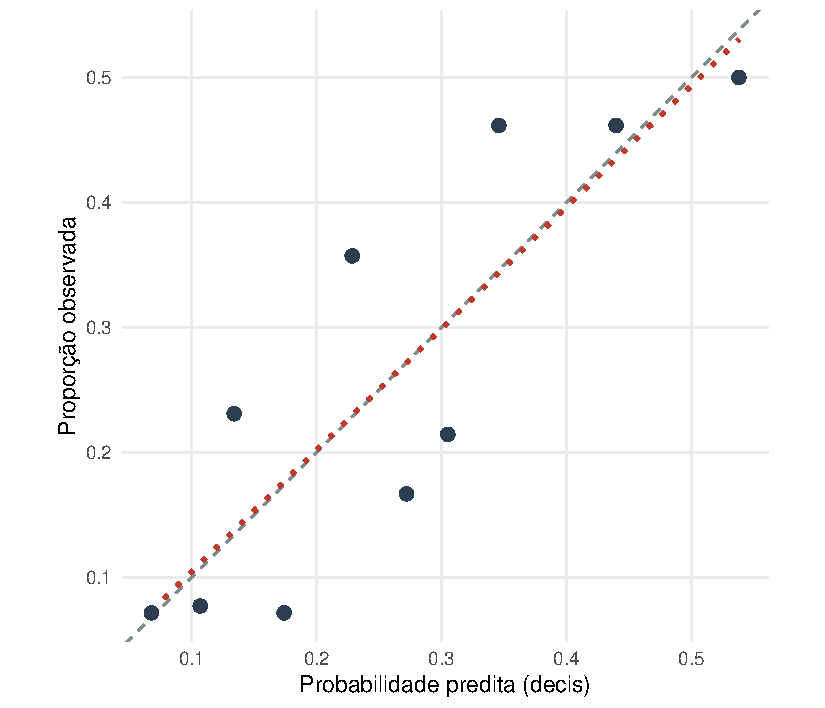
\includegraphics[width=0.8\textwidth]{outputs/figura_calibracao_fibrose.pdf}
  \caption{Calibração do modelo de fibrose (probabilidades observadas vs.
           preditas).}
\end{figure}

\begin{figure}[H]
  \centering
  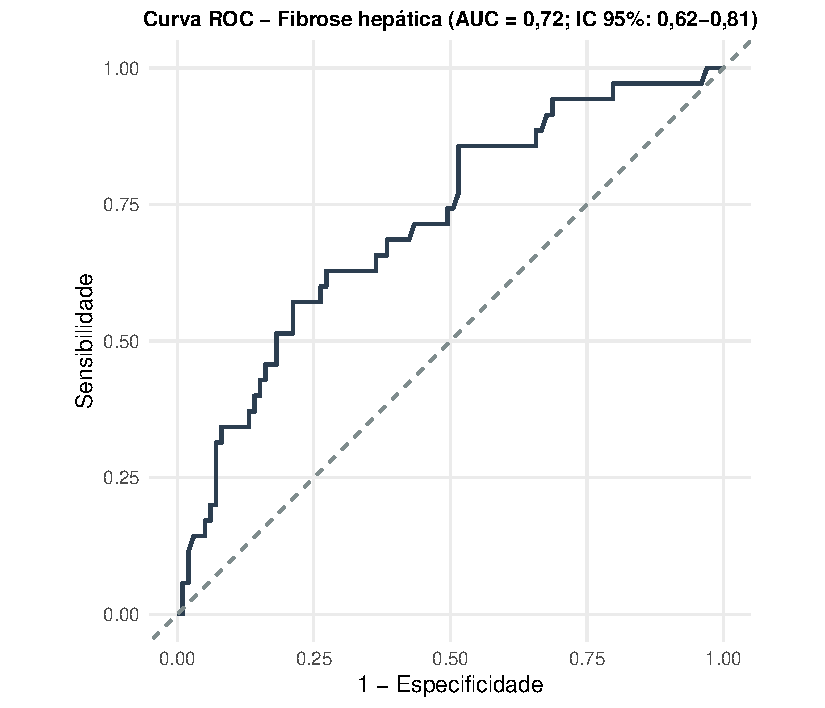
\includegraphics[width=0.8\textwidth]{outputs/figura_roc_fibrose.pdf}
  \caption{Curva ROC do modelo de fibrose hepática.}
\end{figure}

\begin{figure}[H]
  \centering
  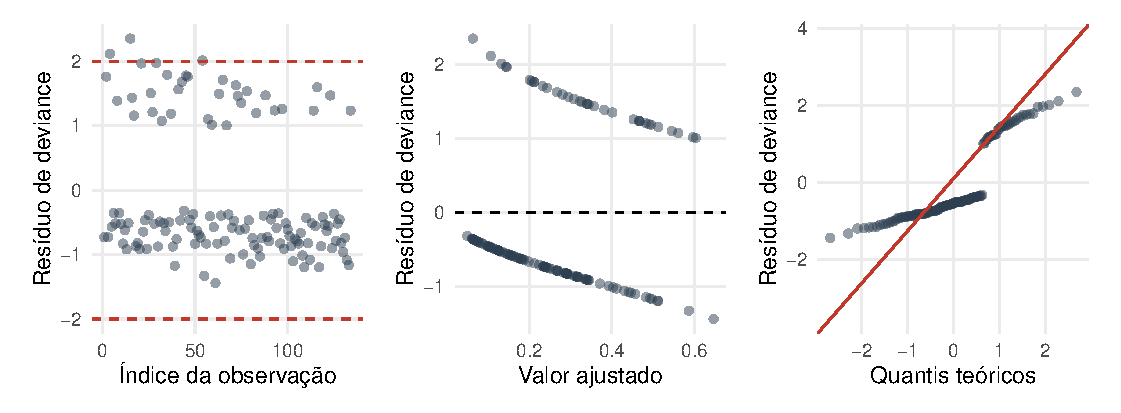
\includegraphics[width=0.8\textwidth]{outputs/figura_residuos_fibrose.pdf}
  \caption{Resíduos de Pearson e Deviance do modelo de fibrose.}
\end{figure}

\begin{figure}[H]
  \centering
  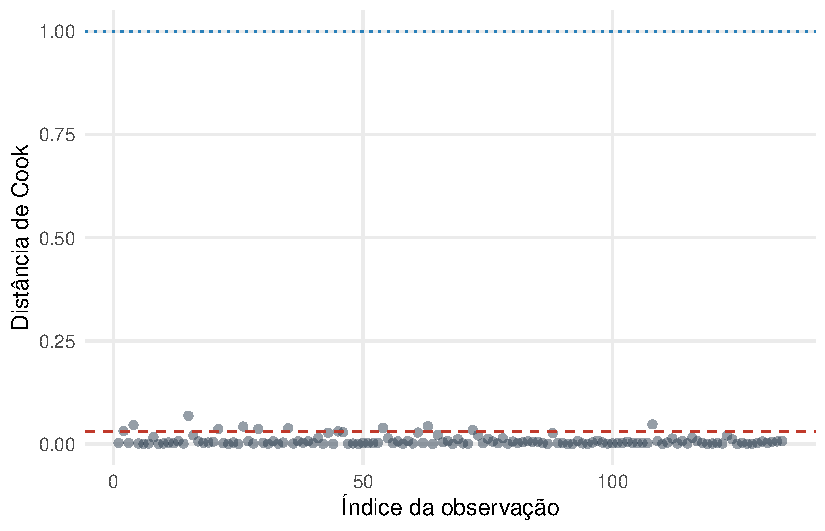
\includegraphics[width=0.8\textwidth]{outputs/figura_cook_fibrose.pdf}
  \caption{Distância de Cook do modelo de fibrose.}
\end{figure}

\begin{figure}[H]
  \centering
  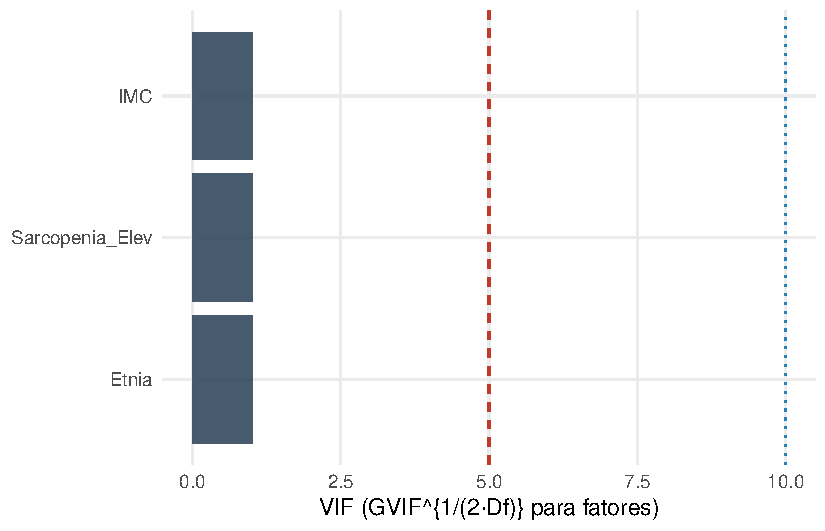
\includegraphics[width=0.8\textwidth]{outputs/figura_vif_fibrose.pdf}
  \caption{VIF/GVIF das covariáveis do modelo de fibrose.}
\end{figure}

\subsection{Modelo de DHEM}

O modelo final de DHEM também apresentou ajuste adequado: Hosmer--Lemeshow com
$X^2 = 2{,}32$ (valor-p = 0,509), AUC = 0,76 (IC 95\%: 0,65--0,88), VIF máximo
de 1,1 e maior distância de Cook de 0,107, sem observações influentes
problemáticas. Assim como no modelo de fibrose, os resíduos não revelaram
padrões sistemáticos relevantes, e a discriminação foi ligeiramente superior.

\begin{figure}[H]
  \centering
  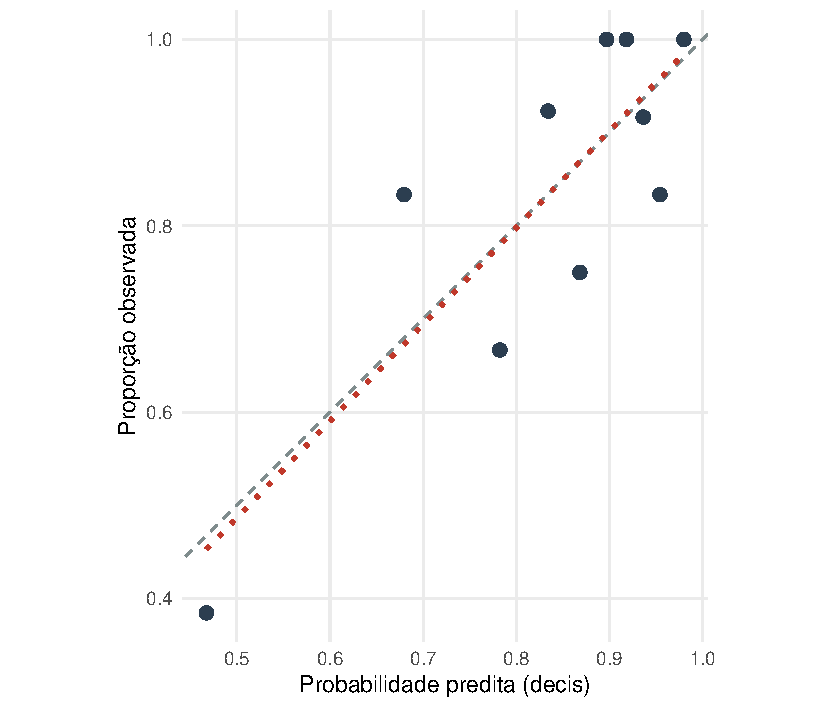
\includegraphics[width=0.8\textwidth]{outputs/figura_calibracao_dhem.pdf}
  \caption{Calibração do modelo de DHEM (probabilidades observadas vs.
           preditas).}
\end{figure}

\begin{figure}[H]
  \centering
  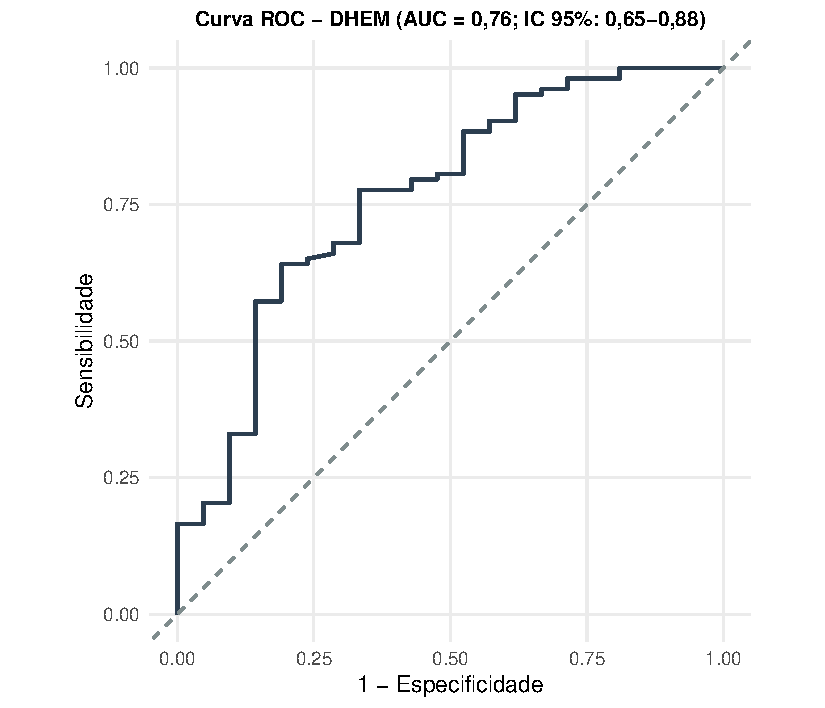
\includegraphics[width=0.8\textwidth]{outputs/figura_roc_dhem.pdf}
  \caption{Curva ROC do modelo de DHEM.}
\end{figure}

\begin{figure}[H]
  \centering
  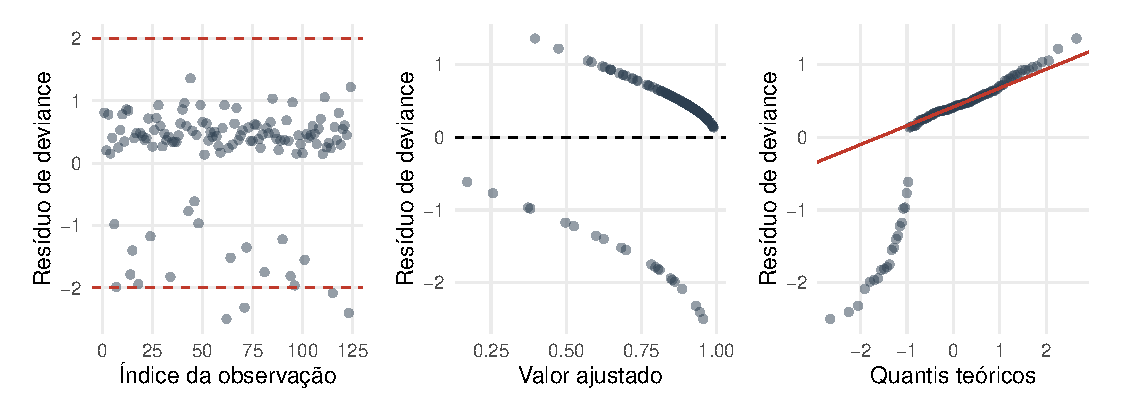
\includegraphics[width=0.8\textwidth]{outputs/figura_residuos_dhem.pdf}
  \caption{Resíduos de Pearson e Deviance do modelo de DHEM.}
\end{figure}

\begin{figure}[H]
  \centering
  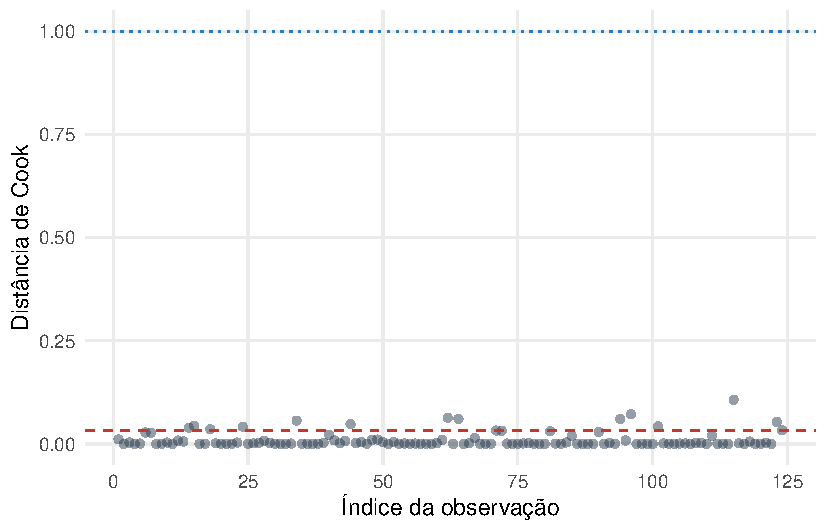
\includegraphics[width=0.8\textwidth]{outputs/figura_cook_dhem.pdf}
  \caption{Distância de Cook do modelo de DHEM.}
\end{figure}

\begin{figure}[H]
  \centering
  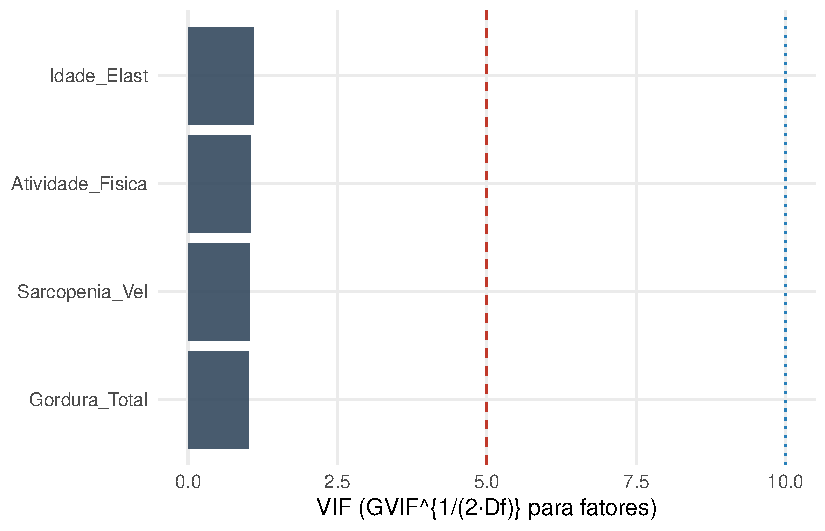
\includegraphics[width=0.8\textwidth]{outputs/figura_vif_dhem.pdf}
  \caption{VIF/GVIF das covariáveis do modelo de DHEM.}
\end{figure}

\subsection{Modelos Lineares de Conversão de MMEA (Concordância)}
\label{sec:apendice_concordancia}

Para cada um dos seis pares de ajustes contínuos de MMEA foram ajustados o
modelo sem intercepto $Y = bX$ e o modelo irrestrito $Y = a + bX$, extraindo-se
as métricas consolidadas na Tabela~\ref{tab:diagnosticos_concordancia}:
coeficiente $b$ com erro padrão (EP), $R^2$ não centrado e RMSE dos resíduos,
teste de Shapiro--Wilk sobre os resíduos de $Y = bX$, teste de significância do
intercepto no modelo irrestrito ($H_0: a = 0$) e máxima distância de Cook.

\begin{table}[H]
  \centering
  \caption{Diagnósticos dos modelos lineares sem intercepto ($Y = bX$) para os
           seis pares de ajustes de MMEA: coeficiente $b$ (EP), $R^2$ não
           centrado, RMSE, teste de Shapiro--Wilk dos resíduos, teste do
           intercepto no modelo irrestrito ($a \neq 0$) e avaliação do ajuste.}
  \label{tab:diagnosticos_concordancia}
  \resizebox{\ifdim\width>\linewidth\linewidth\else\width\fi}{!}{
\begin{tabular}[t]{>{\raggedright\arraybackslash}p{3.2cm}>{\centering\arraybackslash}p{1.9cm}>{\centering\arraybackslash}p{1.5cm}>{\centering\arraybackslash}p{1.5cm}>{\centering\arraybackslash}p{2.7cm}>{\centering\arraybackslash}p{3.1cm}>{\centering\arraybackslash}p{4.0cm}}
\toprule
Par & b (EP) & R$^{2}$ & RMSE & valor-p (SW Resíduos) & valor-p (Intercepto $\neq$ 0) & Avaliação do Ajuste\\
\midrule
\cellcolor{gray!10}{Newman vs Baumgartner} & \cellcolor{gray!10}{0,080 (0,166)} & \cellcolor{gray!10}{0,001} & \cellcolor{gray!10}{7,933} & \cellcolor{gray!10}{0,710} & \cellcolor{gray!10}{< 0,001} & \cellcolor{gray!10}{Inadequado (intercepto $\neq$ 0)}\\
Newman vs FNIH & 0,016 (0,014) & 0,009 & 0,649 & < 0,001 & < 0,001 & Inadequado (intercepto $\neq$ 0; resíduos não normais)\\
\cellcolor{gray!10}{Newman vs MMEA/peso} & \cellcolor{gray!10}{0,262 (0,523)} & \cellcolor{gray!10}{0,002} & \cellcolor{gray!10}{24,948} & \cellcolor{gray!10}{< 0,001} & \cellcolor{gray!10}{< 0,001} & \cellcolor{gray!10}{Inadequado (intercepto $\neq$ 0; resíduos não normais)}\\
Baumgartner vs FNIH & 0,080 (0,001) & 0,949 & 0,147 & < 0,001 & 0,002 & Inadequado (intercepto $\neq$ 0; resíduos não normais)\\
\cellcolor{gray!10}{Baumgartner vs MMEA/peso} & \cellcolor{gray!10}{3,089 (0,046)} & \cellcolor{gray!10}{0,965} & \cellcolor{gray!10}{4,690} & \cellcolor{gray!10}{0,961} & \cellcolor{gray!10}{< 0,001} & \cellcolor{gray!10}{Inadequado (intercepto $\neq$ 0)}\\
FNIH vs MMEA/peso & 37,965 (0,409) & 0,981 & 3,412 & < 0,001 & < 0,001 & Inadequado (intercepto $\neq$ 0; resíduos não normais)\\
\bottomrule
\end{tabular}}

\end{table}

Em todos os pares, o teste do intercepto no modelo irrestrito rejeitou a
hipótese $a = 0$ ($p < 0{,}001$; no par Baumgartner vs FNIH, $p = 0{,}002$),
indicando que a reta que melhor representa a relação contínua entre os métodos
não passa pela origem e que o modelo sem intercepto $Y = bX$ é
estruturalmente inadequado como equação de conversão entre escalas não
comensuráveis. O teste de Shapiro--Wilk rejeitou a normalidade dos resíduos em
quatro dos seis pares (exceções: Newman vs Baumgartner e Baumgartner vs
MMEA/peso), e o painel de resíduos vs.~valores ajustados
(Figura~\ref{fig:residuos_concordancia}) evidencia dispersão residual
crescente com o ajuste (heterocedasticidade) e tendência sistemática da média
residual, confirmando a violação severa dos pressupostos. As violações de
pressupostos indicam que o coeficiente $\hat{b}$ não constitui um fator de
conversão matemática válido entre os métodos, devendo a avaliação de
concordância restringir-se às classificações dicotômicas (coeficientes
Kappa), como discutido na Seção~\ref{sec:obj2}.

\begin{figure}[H]
  \centering
  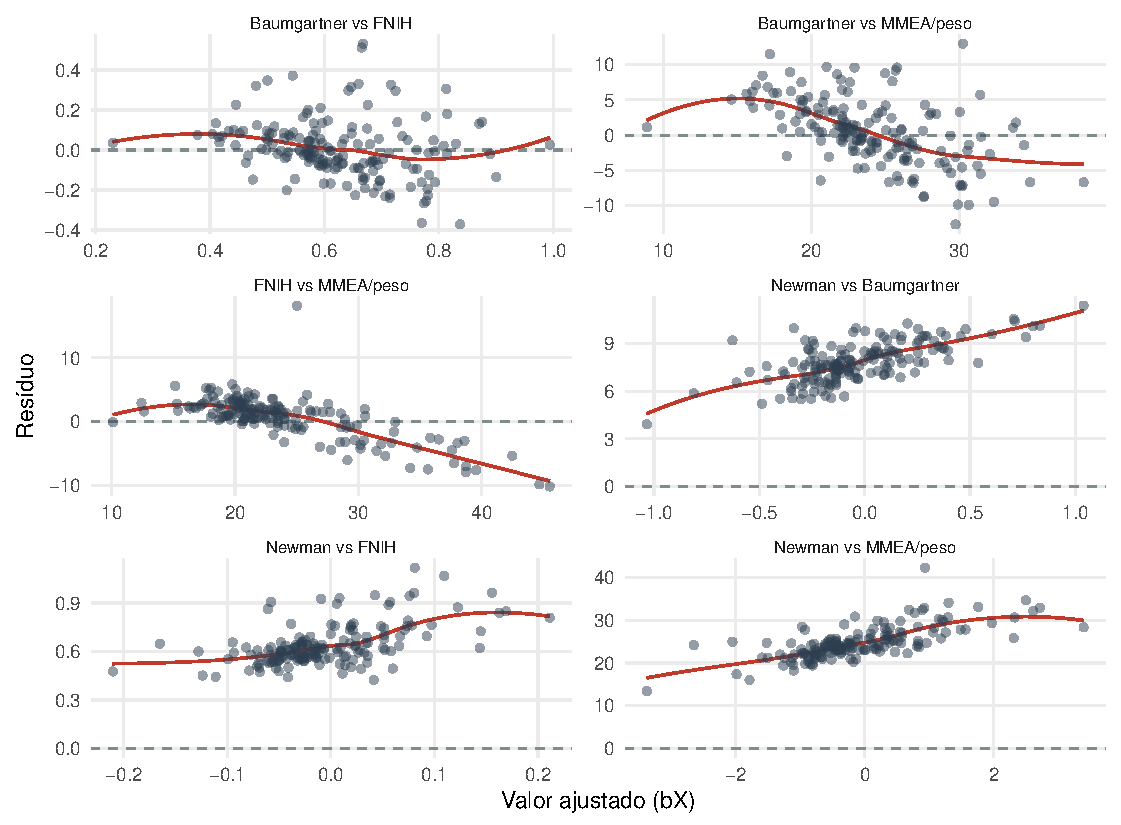
\includegraphics[width=\textwidth]{outputs/figura_residuos_concordancia.pdf}
  \caption{Resíduos vs.~valores ajustados dos modelos sem intercepto $Y = bX$
           para os seis pares de ajustes de MMEA (linha vermelha: suavização
           LOESS).}
  \label{fig:residuos_concordancia}
\end{figure}

\end{document}
